\documentclass[journal=jpcbfk,manusciprt=article]{achemso}

\usepackage{graphicx}
\usepackage{wrapfig}
\usepackage{subcaption}
\usepackage{amsmath} 
\usepackage{siunitx}
\usepackage{booktabs}
\usepackage{gensymb}

%MRS5: could be punchier. I will keep thinking.  I should be the last author.  Chen the names that Joe and Matt wanttu use (presumably with some middle initial?
\title{Understanding the nanoscale structure of hexagonal phase lyotropic 
liquid crystal membranes}
\author{Benjamin J. Coscia}
\author{Richard D. Noble}
\author{Douglas L. Gin}
\affiliation{Department of Chemical and Biological Engineering, University of Colorado Boulder, Boulder, CO 80309, USA}
\alsoaffiliation{Department of Chemistry and Biochemistry, University of Colorado Boulder, Boulder CO 80309, USA}
\author{Joe Yelk}
\author{Matthew Glaser}
\affiliation{Department of Physics, University of Colorado Boulder, Boulder CO, 80309, USA}
\author{Xunda Feng}
\affiliation{Department of Chemical and Environmental Engineering, Yale University, New Haven, Connecticut 06511, USA}
\author{Michael R. Shirts}
\email{michael.shirts@colorado.edu}
\affiliation{Department of Chemical and Biological Engineering, University of Colorado Boulder, Boulder, CO 80309, USA}
\begin{document}

  \graphicspath{{./figures/}}

  \begin{tocentry}
  \end{tocentry}
  
  \begin{abstract}
 
  Nanostructured porous membranes made from the cross-linked hexagonal phase of
  self-assembled lyotropic liquid crystals (LLCs) are a promising material for
  selective separations.  In this work, we develop an atomistic molecular model
  of an LLC membrane. We show that our model is maximally consistent with
  experimental observations by comparing simulated X-ray Diffraction (XRD)
  patterns and calculated ionic conductivity to their experimental counterparts.
  We explore, in depth, the composition and structure of the nanopores in order
  to give insights that are not easily accessible to experimentalists.  The
  clearer picture of the nanoscopic structure of these membranes provided in this
  study will enable a better understanding of the mechanisms of small molecule
  transport within these nanopores.

  \end{abstract}

  \section{Introduction}
 
  %MRS5: want to get people engaged from the beginning. The first paragraph
  %should describe a problem to be solved. Then you can get into the motivating
  %details (like background of the alternatives, and why we need something
  %different).  I feel like this is an introduction into different types of
  %membranes, though it should be an introduction to the problem that this paper
  %takes steps towards solving.
  
  A highly selective membrane would be useful for the recovery of valuable
  products from complex aqueous and organic solutions.  For example, flowback
  water (FW) produced during hydraulic fracturing is a complex wastewater full of
  potentially valuable dissolved organic compounds such as acetate
  \cite{dischinger_application_2017}. There is increasing pressure to reuse
  hydraulic fracturing water rather than dispose of it in order to reduce social
  and environmental impacts as well as cost \cite{theodori_hydraulic_2014}.
  Rather fully than dispose of the wastestream generated in the recycling
  process, we can instead use highly selective membranes in order to successfully
  recover useful compounds. 

%MRS6: I would keep a paragraph about here how current membranes DON'T
%work for this purpose. But one paragraph is enough.x
 
%  The permeability-selectivity tradeoff is a well-known problem in the membrane
%  separations community. It is difficult to increase the permeability of a 
%  desired molecular or atomic species, while maintaining the same retention of
%  an undesired species.

%  Current commercial RO and NF membranes suffer from limitations inherent to
%  their fabrication. Although scalable, each of these two types of membranes has
%  a degree of stochasticity that makes overcoming the permeability-selectivity
%  tradeoff a challenge. Namely, it is difficult to increase the permeability of
%  a desired molecular or atomic species, while maintaining the same retention of
%  an undesired species \cite{werber_materials_2016}. 

%MRS5: under solution-diffusion, then the free energy to partition into the membrane is important as well, correct?
%  Selective separation by a semipermeable membrane barrier can be broken into two
%  steps: barrier entry and transport through the barrier. A solute's ability to
  % BJC: can also come up with a third step: exit. Which I think is mostly chemical potential gradient
%  enter a given membrane barrier is decided by its size, shape, charge, polarity
%  and how those factors combine to interact with the membrane material. The same
%  properties affect the rate at which a solute travels across the barrier. Since
%  undesired solutes may still enter the membrane, their diffusion rates relative
%  to desired solutes are important
%  \cite{gin_polymerized_2008,wijmans_solution-diffusion_1995}. To achieve optimum
%  selectivity, it is necessary to design membranes in a way that one can tune the
%  relative diffusivities of desired and undesired solutes.

  Selective separation by a semipermeable membrane barrier is a function of the
  geometric and chemical interactions of solutes with the membrane material. A
  molecule's size, shape, charge and polarity combine to determine the degree to
  which a solute partitions into a membrane and how fast it travels through the
  membrane. To separate a component from a mixture, one must understand how to
  design membranes in order to tune the relative transport rates of desired and
  undesired solutes\cite{gin_polymerized_2008,wijmans_solution-diffusion_1995}. 

% BJC: Maybe I don't even need to dive into explaining RO and NF.
%  Reverse osmosis (RO) and nanofiltration (NF) are membrane-based separation
%  processes widely used to create potable or reusable water by removing salts and
%  other dissolved compounds from water sources. RO membranes are typically thin
%  film composite (TFC) membranes with a porous support layer and a dense
%  crosslinked polymer active layer which  separates all solutes from water. NF
%  membranes have porous architectures with pores on the order of 1 nm in size
%  which separate primarily based on solute size
%  \cite{van_der_bruggen_review_2003}. 

  Crosslinked lyotropic liquid crystal (LLC) membranes may be capable of
  performing highly selective separations. LLCs are amphiphilic molecules that
  have the ability to self-assemble into porous nanostructures
  \cite{smith_ordered_1997} which can be crosslinked to create mechanically
  strong membrane films with pores on the order of 1 nm in diameter
  \cite{zhou_supported_2005}. Unlike commercial NF membranes, LLC membrane pores
  are uniform in size. Since LLC membranes lack a pore size distribution, they
  inherently exhibit high selectivity due to their strict molecular weight
  cut-off (MWCO)~\cite{zhou_supported_2005}. Additionally, the LLC monomers
  %MRS6:
  described in this paper
  %chosen to make membranes for this application 
  are salts, and therefore lead to
  Donnan exclusion of ions in solution. The membrane gains a net surface charge
  when counterions from head groups that line the pore walls escape into the feed
  solution in order to balance the gradients of concentration and electric
  potential \cite{donnan_theory_1995}.    

  The feasibility of LLC membranes has been demonstrated using LLCs that form
  the type 1 bicontinuous cubic (Q\textsubscript{I})
  \cite{hatakeyama_water_2011,hatakeyama_nanoporous_2010,carter_glycerol-based_2012},
  and the inverted hexagonal (H\textsubscript{II}) \cite{zhou_supported_2005}
  phases (See Figure~\ref{fig:bcc_v_hII}). When separating organic solutes from
  NaCl, Q\textsubscript{I} phase membrane filtration experiments have shown
  selectivity 2--3 times higher than commercial RO and 6--12 times higher than
  commercial NF membranes \cite{dischinger_application_2017}.  When separating a
  series of various sized dyes, the H\textsubscript{II} phase membrane showed
  complete rejection of dyes bigger than 1.2 nm in size
  \cite{zhou_supported_2005}. 

  The H\textsubscript{II} phase pore geometry is 
%MRS6:
%better 
has a higher theoretical capacity
for transport than the
  Q\textsubscript{I} phase. The H\textsubscript{II} phase forms at room
  temperature in the presence of c.a.~10 wt\% water and consists of hexagonally
  packed, hydrophilic pore columns\cite{smith_ordered_1997}. In the absence of
  water, neat monomer will form the same hexagonal columnar structure which, in
  literature, has been referred to as the Col\textsubscript{h} thermotropic
  phase\cite{feng_scalable_2014} (See Figure~\ref{fig:hII_phase}).  The most
  promising Q\textsubscript{I} phase for membrane applications forms at 70\degree
  C when monomer is mixed with c.a.~20 wt\%
  glycerol\cite{carter_glycerol-based_2012}. Q\textsubscript{I} phase membranes
  consist of a tortuous network of three dimensionally interconnected pores that
  prevent optimal through-plane transport. The densely packed, non-tortuous and
  uniform sized pores of H\textsubscript{II} phase membranes represents the ideal
  geometry for achieving high solute flux\cite{matyka_tortuosity-porosity_2008}.
  Despite the promise of the H\textsubscript{II} phase, the hexagonally packed
  liquid crystalline domains, formed during self-assembly of NA-GA3C11 monomers, are
  isotropically aligned which is detrimental to membrane performance. 

%MRS5: maybe less about Q_I since it's not in this paper?  The introduction should be an introduction to the paper.
%  The most promising Q\textsubscript{I} phase for membrane
%  applications forms at 70\degree C when monomer is mixed with c.a.~20 wt\%
%  glycerol\cite{carter_glycerol-based_2012}. The Q\textsubscript{I} phase
%  consists of a network of three dimensionally interconnected pores (See
%  Figure~\ref{fig:bcc_phases}). This complex geometry effectively adds a degree
%  of tortuosity to the membrane which prevents optimal through-plane transport.
%  Despite the geometric differences between the Q\textsubscript{I} and
%  H\textsubscript{II} phase, the chemical environment within the pores is
%  expected to be similar, and either membrane should be highly selective. 

  % BJC: I like this figure, but I don't know if it is necessary in the main body. i  % Maybe move to supplemental. Thoughts?
  \begin{figure}
  \centering
  \begin{subfigure}{0.45\textwidth}
        \centering
        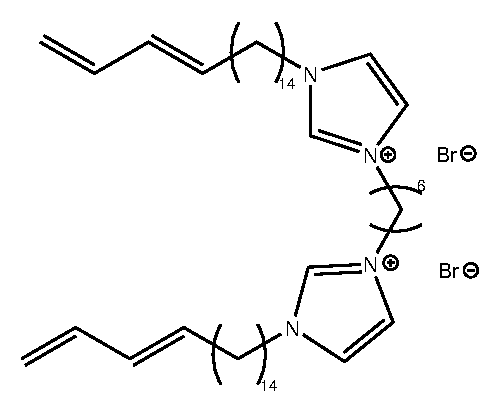
\includegraphics[trim=-2cm 0 0 0, clip, height=4.5cm]{Dibrpyr14.eps}
        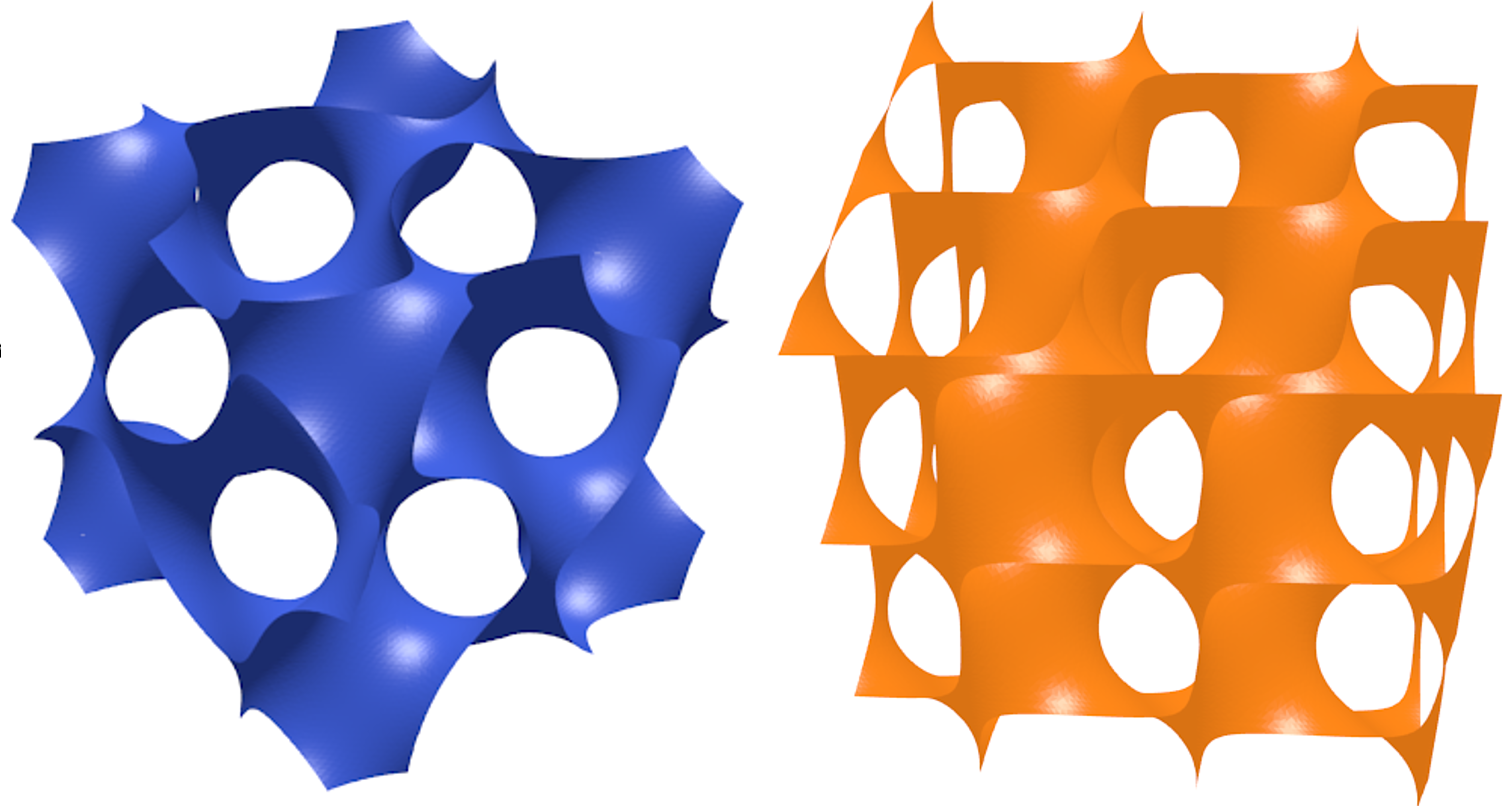
\includegraphics[height=4.5cm]{bcc_phases.png}
        \caption{}\label{fig:bcc_phases}
  \end{subfigure}
  \hspace{1cm}
  \begin{subfigure}{0.45\textwidth}
        \centering
        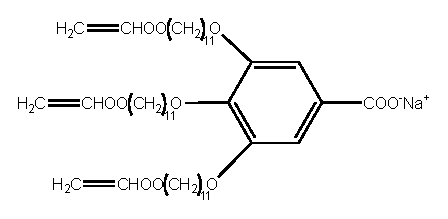
\includegraphics[trim=0 -0.5cm 0 -0.5cm, clip, height=4.5cm]{NaGA3C11.eps}
        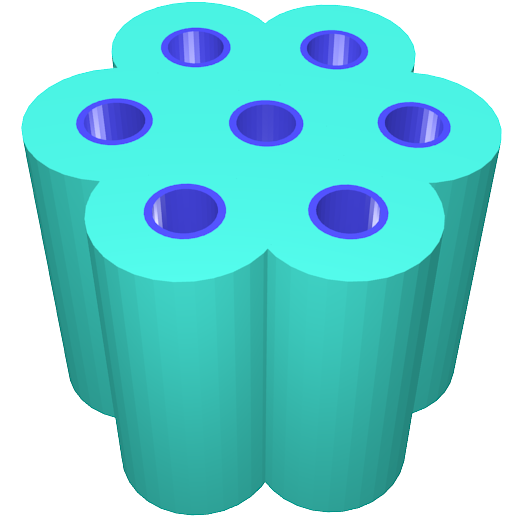
\includegraphics[height=4.5cm]{hexagonal_packing.png}
        \caption{}\label{fig:hII_phase}
  \end{subfigure}
%MRS5: not sure Q should be in here.
  \caption{The choice of LLC monomer and solvent leads to different accessible liquid
        crystalline phases. The monomer shown in (a) forms the Q\textsubscript{I} phase
        in either the Ia3d (left) or Pn3m (right) space group. The surfaces shown
        represent the interface between the hydrophilic and hydrophobic regions of the unit
        cell. As pictured, we assume that each region occupies an equal volume. The
        monomer shown in (b) will form the hexagonal columnar phase
        (H\textsubscript{II} in the presence of water or Col\textsubscript{h} when no
         water is present) The blue region represent the hydrophilic pores while the cyan region represents the surrounding hydrophobic monomer tails.}\label{fig:bcc_v_hII}
  \end{figure}


  %Nanostructured porous membrane materials have become increasingly popular for
  %aqueous separations applications such as desalination and biorefinement because
  %they offer the ability to control pore architecture at the molecular scale,
  %thereby permitting the design of solute-specific separation membranes
  %\cite{humplik_nanostructured_2011}. One can acheive most membrane-based aqueous separations of
  %small molecules using reverse osmosis (RO) or nanofiltration
  %(NF) \cite{van_der_bruggen_review_2003}. While RO and NF have seen many
  %advances in the past few decades, they are far from perfect separation
 

   %MRS4: these two paragraphs are perhaps not ideal.  They describe the process
  %of making the membranes, but that is not what we need as the introduction to
  %THIS paper.  Instead, you need to focus on the strength/issues with RO and
  %NF that motivate this research.
  % BJC3: The point I am trying to make is that the way the membranes are made 
  % results in either low selectivity or low permeability. I could just state
  % that, or give a little background on the processes to make the point more
  % tangible

  %Commercial RO membranes are typically dense thin-film composite (TFC)
  %membranes with a porous support layer and an active layer made of a polymer
  %matrix formed through interfacial polymerization \cite{jeong_interfacial_2007}.
  %During interfacial polymerization, a step-growth polymerization reaction occurs
  %at the interface of an aqueous monomer solution that has been soaked into the
  %support layer, and an organic solution of a second monomer. The polymer matrix
  %is dense and highly cross-linked which gives high rejections but low
  %permeability. 

  %During membrane fabrication,
  %aqueous diamine solution is allowed to penetrate into the polysulfone support
  %layer which is then immersed in trimesoyl chloride, a compound that is
  %immiscible in water. Diamine polymerizes with trimesoyl chloride at the
  %solution interface and creates a thin film that physically adheres to the
  %polysulfone support. 
 
%  solution.  Through the use of a non-solvent, a polymer-rich and polymer-poor
%  phase is formed. A membrane is created as the polymer-poor phase forms pores in
%  the polymer-rich phase. 
%  During phase inversion, a thin polymer film is precipitated out of a polymer

%  NF membranes are typically porous membranes made by a phase-inversion
%  process. The most widely used phase-inversion process is immersion
%  precipitation, during which one submerges a polymer, dissolved in a solvent, in
%  a non-solvent. A solid, porous polymer membrane is all that remains once all
%  solvent has been removed by non-solvent exchange
%  \cite{smolders_microstructures_1992}.  The resultant pores are polydisperse in
%  size, which hurts membrane selectivity. A second technique used to create NF
%  membranes is call track-etching in which a polymer film is bombarded with
%  charged particles, then chemically etched to create pores
%  \cite{apel_track_2001}. The pores are uniform, which benefits selectivity;
%  however, the membranes have a low porosity and subsequently low permeability. 
 
%MRS3: this is a little disconnected to the contents as well.  You want
%the paper to explain the why of doing this research.  Paragraph gives background, but doesn't motivate. 

%  Current commercial RO membranes are thin film composite membranes with a
%  porous support layer and an active layer made of a dense polymer matrix. The
%  membranes are unstructured with tortuous and polydisperse diffusion pathways.
%  Separation occurs based on differences in solubility and diffusivity of solutes
%  within the polymer matrix \cite{wijmans_solution-diffusion_1995}. With
%  optimization, one can exploit these differences to create a functional
%  selective barrier. RO operation costs are suboptimal because high feed
%  pressures are required in order to achieve a useful solvent flux. 

  %BJC : I don't know that this paragraph fits.  
  %MRS3: not really. Maybe take a look at Osuji's recent review (2016, I think) that addresses applications of nanostructured membranes and uses.  Could rewrite the introduction to be more about the general possibilities of nanostructured membranes, not just desalination.  It should be an introduction to what you will talk about in the paper, not to everything related.
 % Improved RO membranes can make desalination more sustainable. Only 0.5\% of
 % the world's water is fresh. Desalination is an important source of potable
 % water, necessary in order to keep up with demand generated by a rapidly growing
 % global population. Although RO is currently the cheapest form of desalination,
 % the cost must be further decreased in order to meet demand. A typical seawater
 % desalination process requires feed pressures in the range of 800 to 1000 psi
 % \cite{fritzmann_state---art_2007}. By designing better membranes for
 % desalination, we can achieve higher water fluxes and reduce feed pressure
 % requirements which will decrease the cost of fresh water production.
 % \cite{humplik_nanostructured_2011}.  

  % financially straining developing regions and contributing strongly to
  % CO\textsubscript{2} emissions. \cite{mcginnis_global_2008} Moreover,
  % designing RO membranes to achieve targeted separations of specific solutes
  % in a complex feed solution is nearly impossible

  %NF was introduced as an intermediate between RO and ultrafiltration, having
  %the ability to separate organic matter and salts on the order of one nanometer
  %in size. Explicit pore pathways running through the thickness of the membrane
  %permit high solvent fluxes at lower pressures than RO. NF membranes typically
  %have a surface charge resulting from ionizable groups which affords separation
  %of ions smaller than the pore radius by the mechanism of Donnan exclusion
  %\cite{van_der_bruggen_review_2003}. NF is often used as a precursor to reverse
  %osmosis since it can efficiently remove a significant portion of dissolved
  %solutes. Following NF pretreatment, RO can further purify the permeate. 
  %Unfortunately, NF membranes, like RO, possess a pore size
  %distribution which limits their ability to perform precise separations
  %\cite{bowen_modelling_2002}. 

%  The permeability-selectivity tradeoff has the potential to be overcome by
%  designing membranes at the molecular level. Next-generation nanoporous
%  membranes with high selectivity, permitted by a precisely controlled pore size,
%  and high permeability, allowed by its porous architecture, have the potential to
%  replace traditional RO and NF membrane technologies. 

%MRS3: I think that this paragraph probably should be couched in terms of what they COULD do, since are not widely used yet.
%MRS3: if talking about existing membranes, should cite performance.
%  Nanostructured membranes can bypass many of the performance issues which
%  plague traditional NF and RO membranes. One can accomplish targeted separations
%  with high selectivity by tuning shape, size and functionality of the molecular
%  building blocks which form these materials. As a result, solute rejecting pores
%  can have their sizes tuned uniformly, resulting in strict size cut-offs.
%  Entirely different mechanisms may govern transport in a given nanostructured
%  material which can inspire novel separation techniques.

%  Development of nanostructured porous materials has been limited by the
%  ability to synthesize and scale various fundamentally sound technologies.
%  Graphene sheets are atomically thick which results in excellent water
%  permeability but defects during manufacturing severely impact selectivity
%  \cite{cohen-tanugi_multilayer_2016}. Molecular dynamics (MD) simulations of
%  carbon nanotubes show promise \cite{humplik_nanostructured_2011}, but synthetic
%  techniques are unable to achieve scalable alignment and pore monodispersity
%  \cite{hata_water-assisted_2004,maruyama_growth_2005}. Zeolites have sub-nm
%  pores with a narrow pore size distribution, and MD simulations of these
%  materials show that they exhibit complete rejection of solvated ions
%  \cite{murad_molecular_1998}- however, experimental rejection was low and
%  attributed to interstitial defects formed during membrane synthesis
%  \cite{li_desalination_2004}. Consequently, there is a need for a scalable
%  nanostructured porous membrane. 

%  Polymeric membranes based on self-assembling lyotropic liquid crystals (LLCs)
%  are suitable candidates for aqueous separation applications. LLCs are
%  amphiphilic molecules that share the characteristic ability of nanostructured
%  porous membrane materials to create highly ordered nanostructures with the
%  added benefits of low cost and synthetic techniques feasible for large-scale
%  production \cite{feng_scalable_2014}. LLC systems created by the monomer
%  Na-GA3C11 (Fig.~\ref{fig:monomer}) have been extensively studied experimentally
%  \cite{feng_scalable_2014,smith_ordered_1997,zhou_supported_2005,resel_h2-phase_2000,feng_thin_2016}.
%  The neat Na-GA3C11 monomer forms the thermotropic liquid crystalline (TLC)
%  Col\textsubscript{h} phase (Fig.\ref{fig:assembly}). The presence of ca. 10
%  wt\% added water results in formation of the lyotropic H\textsubscript{II}
%  phase. In both cases, Na-GA3C11 monomers assembles into mesophases made of
%  hexagonally packed, uniform size, cylinders with hydrophilic head groups
%  oriented inward towards the cylinder center. This LLC assembly is then
%  polymerized in situ to form a cross-linked polymer network to stabilize the
%  structure. The hydrophilic region can act as a pore for aqueous separations
%  \cite{zhou_supported_2005}.  One can envision tailoring the pore region for
%  specific separations by changing the monomer chemistry
%  \cite{resel_h2-phase_2000}.

%MRS5: not a strong thesis.  Why has it been revived?  The reasons for that would be a better thesis.
  Recently, researchers have learned how to macroscopically align the hexagonal
  domains which has revived research into H\textsubscript{II} phase LLC membranes.
%  Research into the H\textsubscript{II} phase of polymerized LLC membranes has
%  been revived in recent years. 
%  During early stages of exploration, hexagonal
%  mesophases formed by Na-GA3C11 (Figure~\ref{fig:assembly}) could not be
%  macroscopically aligned, resulting in low flux membranes, and no clear route
%  towards scalable and economical filtration. 
%  For this reason, research efforts
  Previously, research efforts were focused on the Q\textsubscript{I} phase,
  whose geometry does not require alignment. In 2014, Feng et al.~showed that one
  can align Col\textsubscript{h} hexagonal domains using a magnetic field with
  subsequent cross-linking to lock the structure in place
  \cite{feng_scalable_2014}. In 2016, Feng et al. showed that one could obtain
  the same result using a second technique termed soft confinement
  \cite{feng_thin_2016}. Current efforts are focused on extending the method to
  the H\textsubscript{II} phase and characterizing the performance of these newly
  aligned systems.

  % BJC: Not sure this figure needs to be in the paper. 
  %MRS2: good question.  It helps give people context, which is necessary to
  %move forward.  Perhaps leave it in for now, though may need to get
  %permission to reprint it.
  %\begin{figure} \centering
  %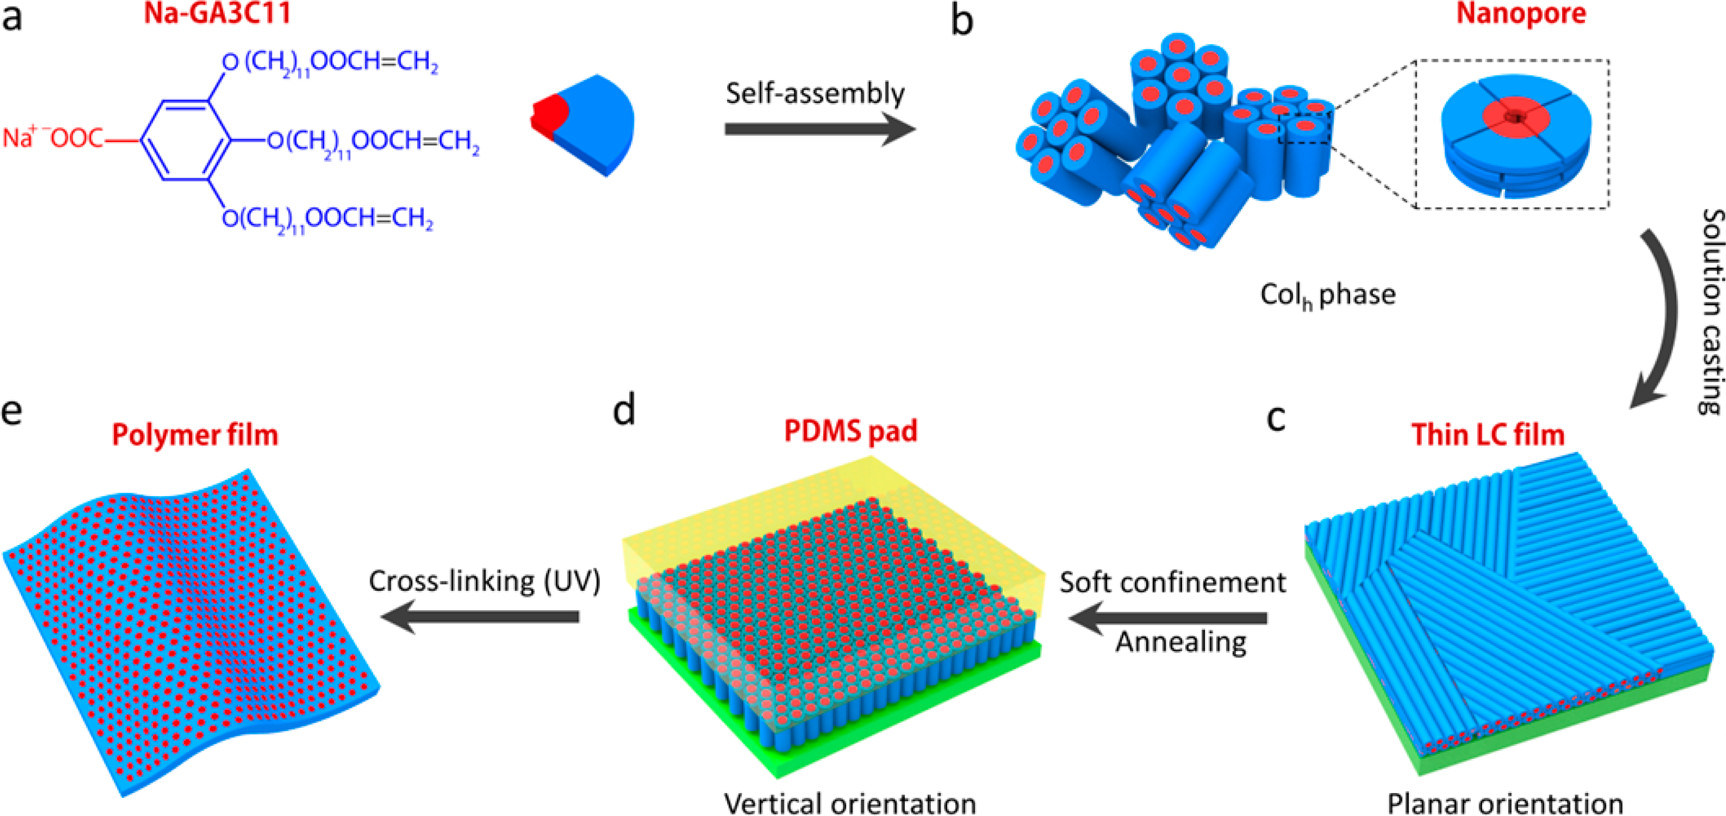
\includegraphics[width=\linewidth]{soft_confinement.png} \caption{The wedge
  %	  shaped liquid crystal monomer (a) self assembles into mesophases with
%		  hexagonally packed pores (b). The pores are made of stacked monomer disks. A
%		  sub-micron-thick film is created by casting a dilute solution of Na-GA3C11/THF
%		  solution onto a silicon substrate and and allowing the solvent to evaporate.
%		  The thin film contains nanoporous columns which lie parallel to the film plane.
%		  (d) When a soft PDMS pad is imposed to the thin film, with subsequent thermal
%		  annealing, the columns align perpendicular to the film plane. (e)
%		  Photo-cross-linking of the aligned film creates a mechanically stable thin film
%		  with vertically aligned nanopores}~\label{fig:soft} \end{figure}

  %BJC: Made my own version of the above, leaving out alignment details since it'

  %BJC: TODO: Scalable vector graphic for monomer structure, make bigger. Convert .svg to .eps
  %           Thicken slabs
  %           Make pore region on slab (blue) bigger
  %           Bump up atom sizes in atomistic render
  \begin{figure}
	\centering
	\begin{subfigure}{.3\textwidth}
		\centering
		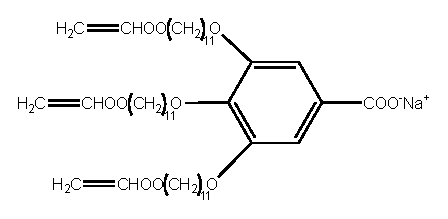
\includegraphics[width=\textwidth]{NaGA3C11.eps}
		\caption{}~\label{fig:monomer}
	\end{subfigure}
	\begin{subfigure}{.3\textwidth}
		\centering
		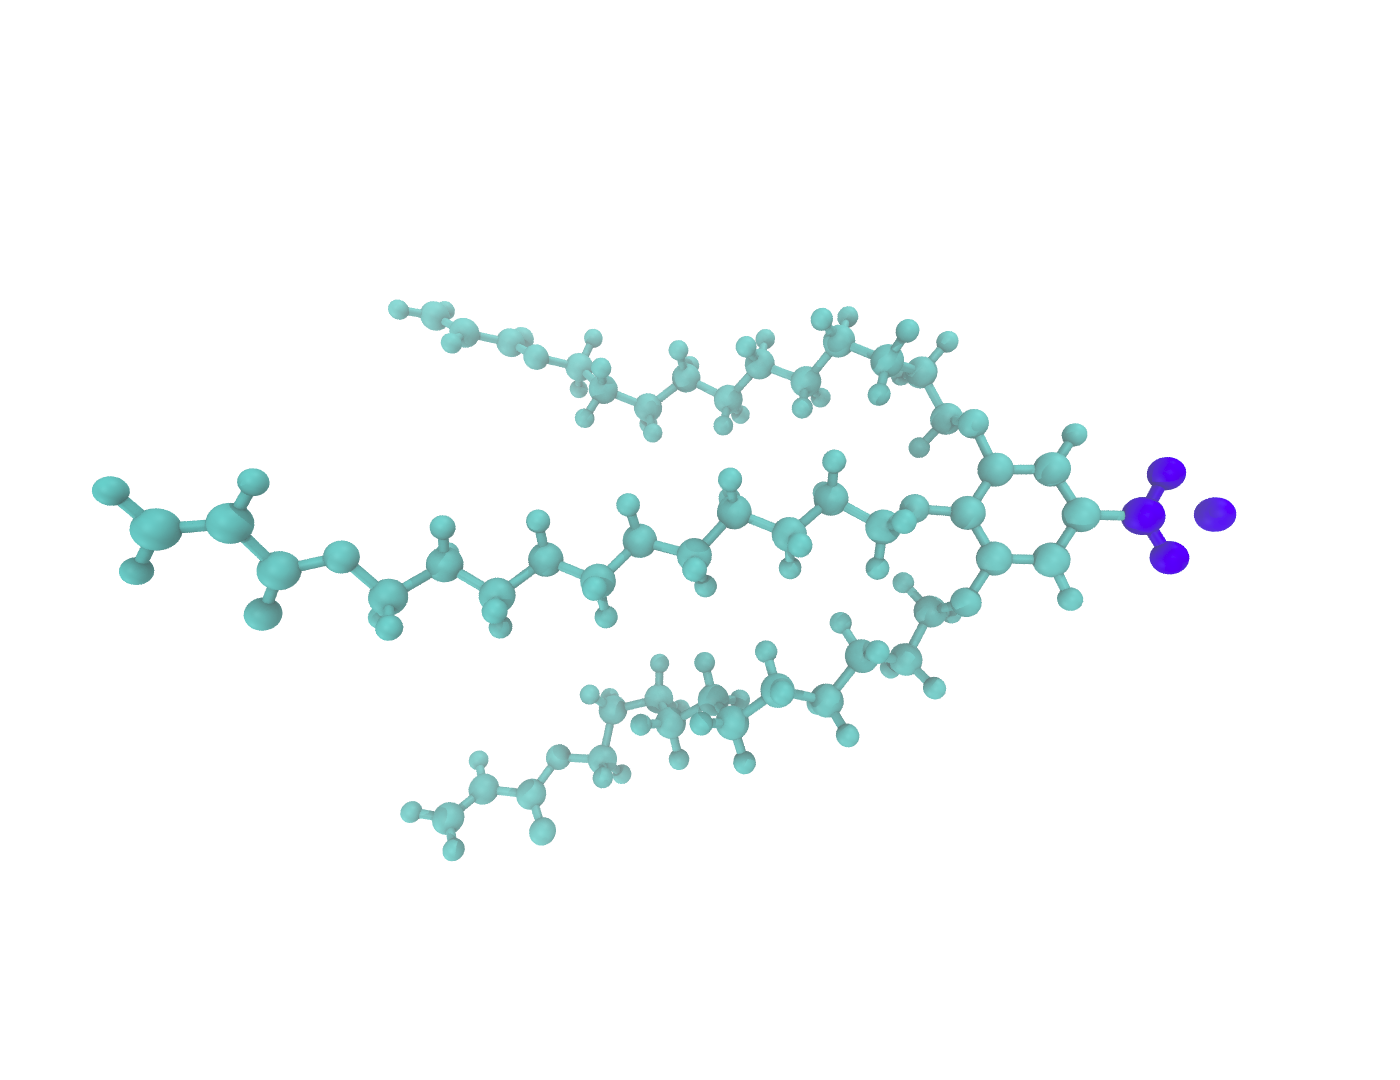
\includegraphics[width=\textwidth]{monomer_twocolor.png}
		\caption{}~\label{fig:atomistic_monomer}
	\end{subfigure}
	\begin{subfigure}{0.3\linewidth}
		\centering
		
\includegraphics[width=\textwidth]{wedge_thick.png}
		\caption{}~\label{fig:wedge}
	\end{subfigure}
		\begin{subfigure}{0.4\linewidth}
		\centering
		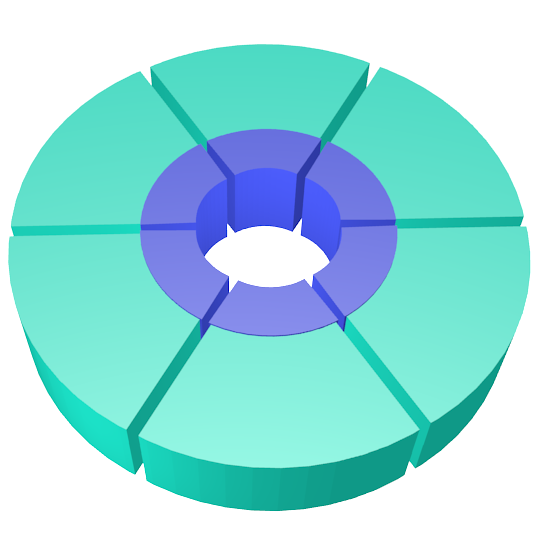
\includegraphics[width=\textwidth]{layer_thick.png}
		\caption{}~\label{fig:wedge_layer}
	\end{subfigure}
	\begin{subfigure}{0.4\linewidth}
		\centering
		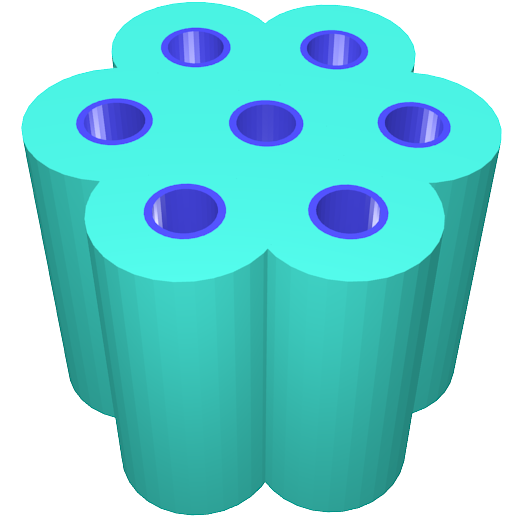
\includegraphics[width=\textwidth]{hexagonal_packing.png}
		\caption{}~\label{fig:hex_packing_simple}
	\end{subfigure}
	\caption{The LLC monomer Na-GA3C11 (a) rendered atomistically (b)
	exhibits wedge-like character (c). Monomer wedges assemble into disks (d) with
	hydrophilic head groups (blue) facing towards the disk center. The disks
	assemble into hexagonally packed columnar mesophases (e).}~\label{fig:assembly}
  \end{figure}

  Our current understanding of 
%MRS6:
the molecular details of
LLC membrane 
%systems 
nanostructure
is not 
%MRS6: 
%rich enough to be
sufficient
  able to precisely design them for specific separations. Over the past 20 years,
  H\textsubscript{II}-phase LLC polymer membrane studies have been limited
  primarily to Na-GA3C11 with some characterization done after minor structural
  modifications. Resel et al.~varied the length of the monomer tails and the
  counterion used and observed its affect on pore spacing
  \cite{resel_structural_2000}. In a later study of rejection performance, it was
  shown that membranes formed by cross-linked Na-GA3C11 in the
  H\textsubscript{II} phase cannot separate solutes less than 1.2 nm in diameter
  because the pores are too large \cite{zhou_supported_2005}. We do not yet
  understand how to controllably reduce the effective pore size or how to tune
  the chemical environment in the nanopores of this or related materials for
  small molecule separations. The only source of predictive modeling for LLC
  systems have been macroscopic models that likely do not adequately describe
  transport at these length scales \cite{hatakeyama_water_2011}. It will be
  challenging to efficiently narrow down the large design space in a laboratory
  setting without a robust model.

  A molecular-level understanding of LLC polymer membrane structure, enabled by
  molecular dynamics (MD) simulations, can provide guidelines to reduce the large
  chemical space available to design monomers for creation of separation-specific
  membranes. A good molecular model should incorporate a detailed picture of the
  nanoscopic pore structure which will be crucial to understanding the role of
  monomer structure in solute transport and membrane design. Models resulting
  from molecular dynamics simulations will provide the required level of detail
  (Fig. \ref{fig:detail}), assuming the force fields are sufficiently accurate.
  With such an atomistic model, we can directly observe molecular-level solute
  transport and suggest governing mechanisms. We can observe how the choice of
  head group interacts with solutes of interest. We can interchange
  counterions which may influence both the pore size and the strength of the
  Donnan potential 

  %which affects the degree to which the membrane can exclude
  %charged species at the membrane surface. 

  In this study, we build a significantly more realistic atomistic model of LLC
  membranes than, to our knowledge, has ever previously been created, and explore
  what new structural information can be gained and what structure hypotheses are
  supported by this model. We validate the model using as much experimental
  information as possible. We are most interested in reproducing the conclusions
  about structure drawn from small angle X-ray scattering (SAXS)
  and wide angle X-ray scattering (WAXS) experiments as well as in matching ionic
  conductivity measurements \cite{feng_thin_2016}.

  \begin{figure}
  \centering
	\begin{subfigure}{0.45\linewidth}
		\centering
		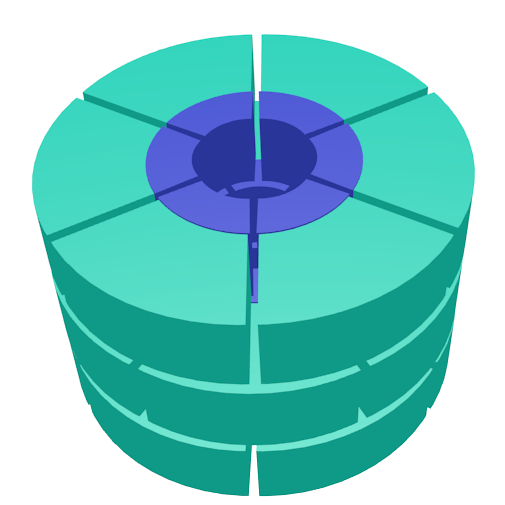
\includegraphics[width=\textwidth]{cartoon_pore.png}
		\caption{}~\label{fig:undetailed_pore}
	\end{subfigure}
	\begin{subfigure}{0.45\linewidth}
		\centering
		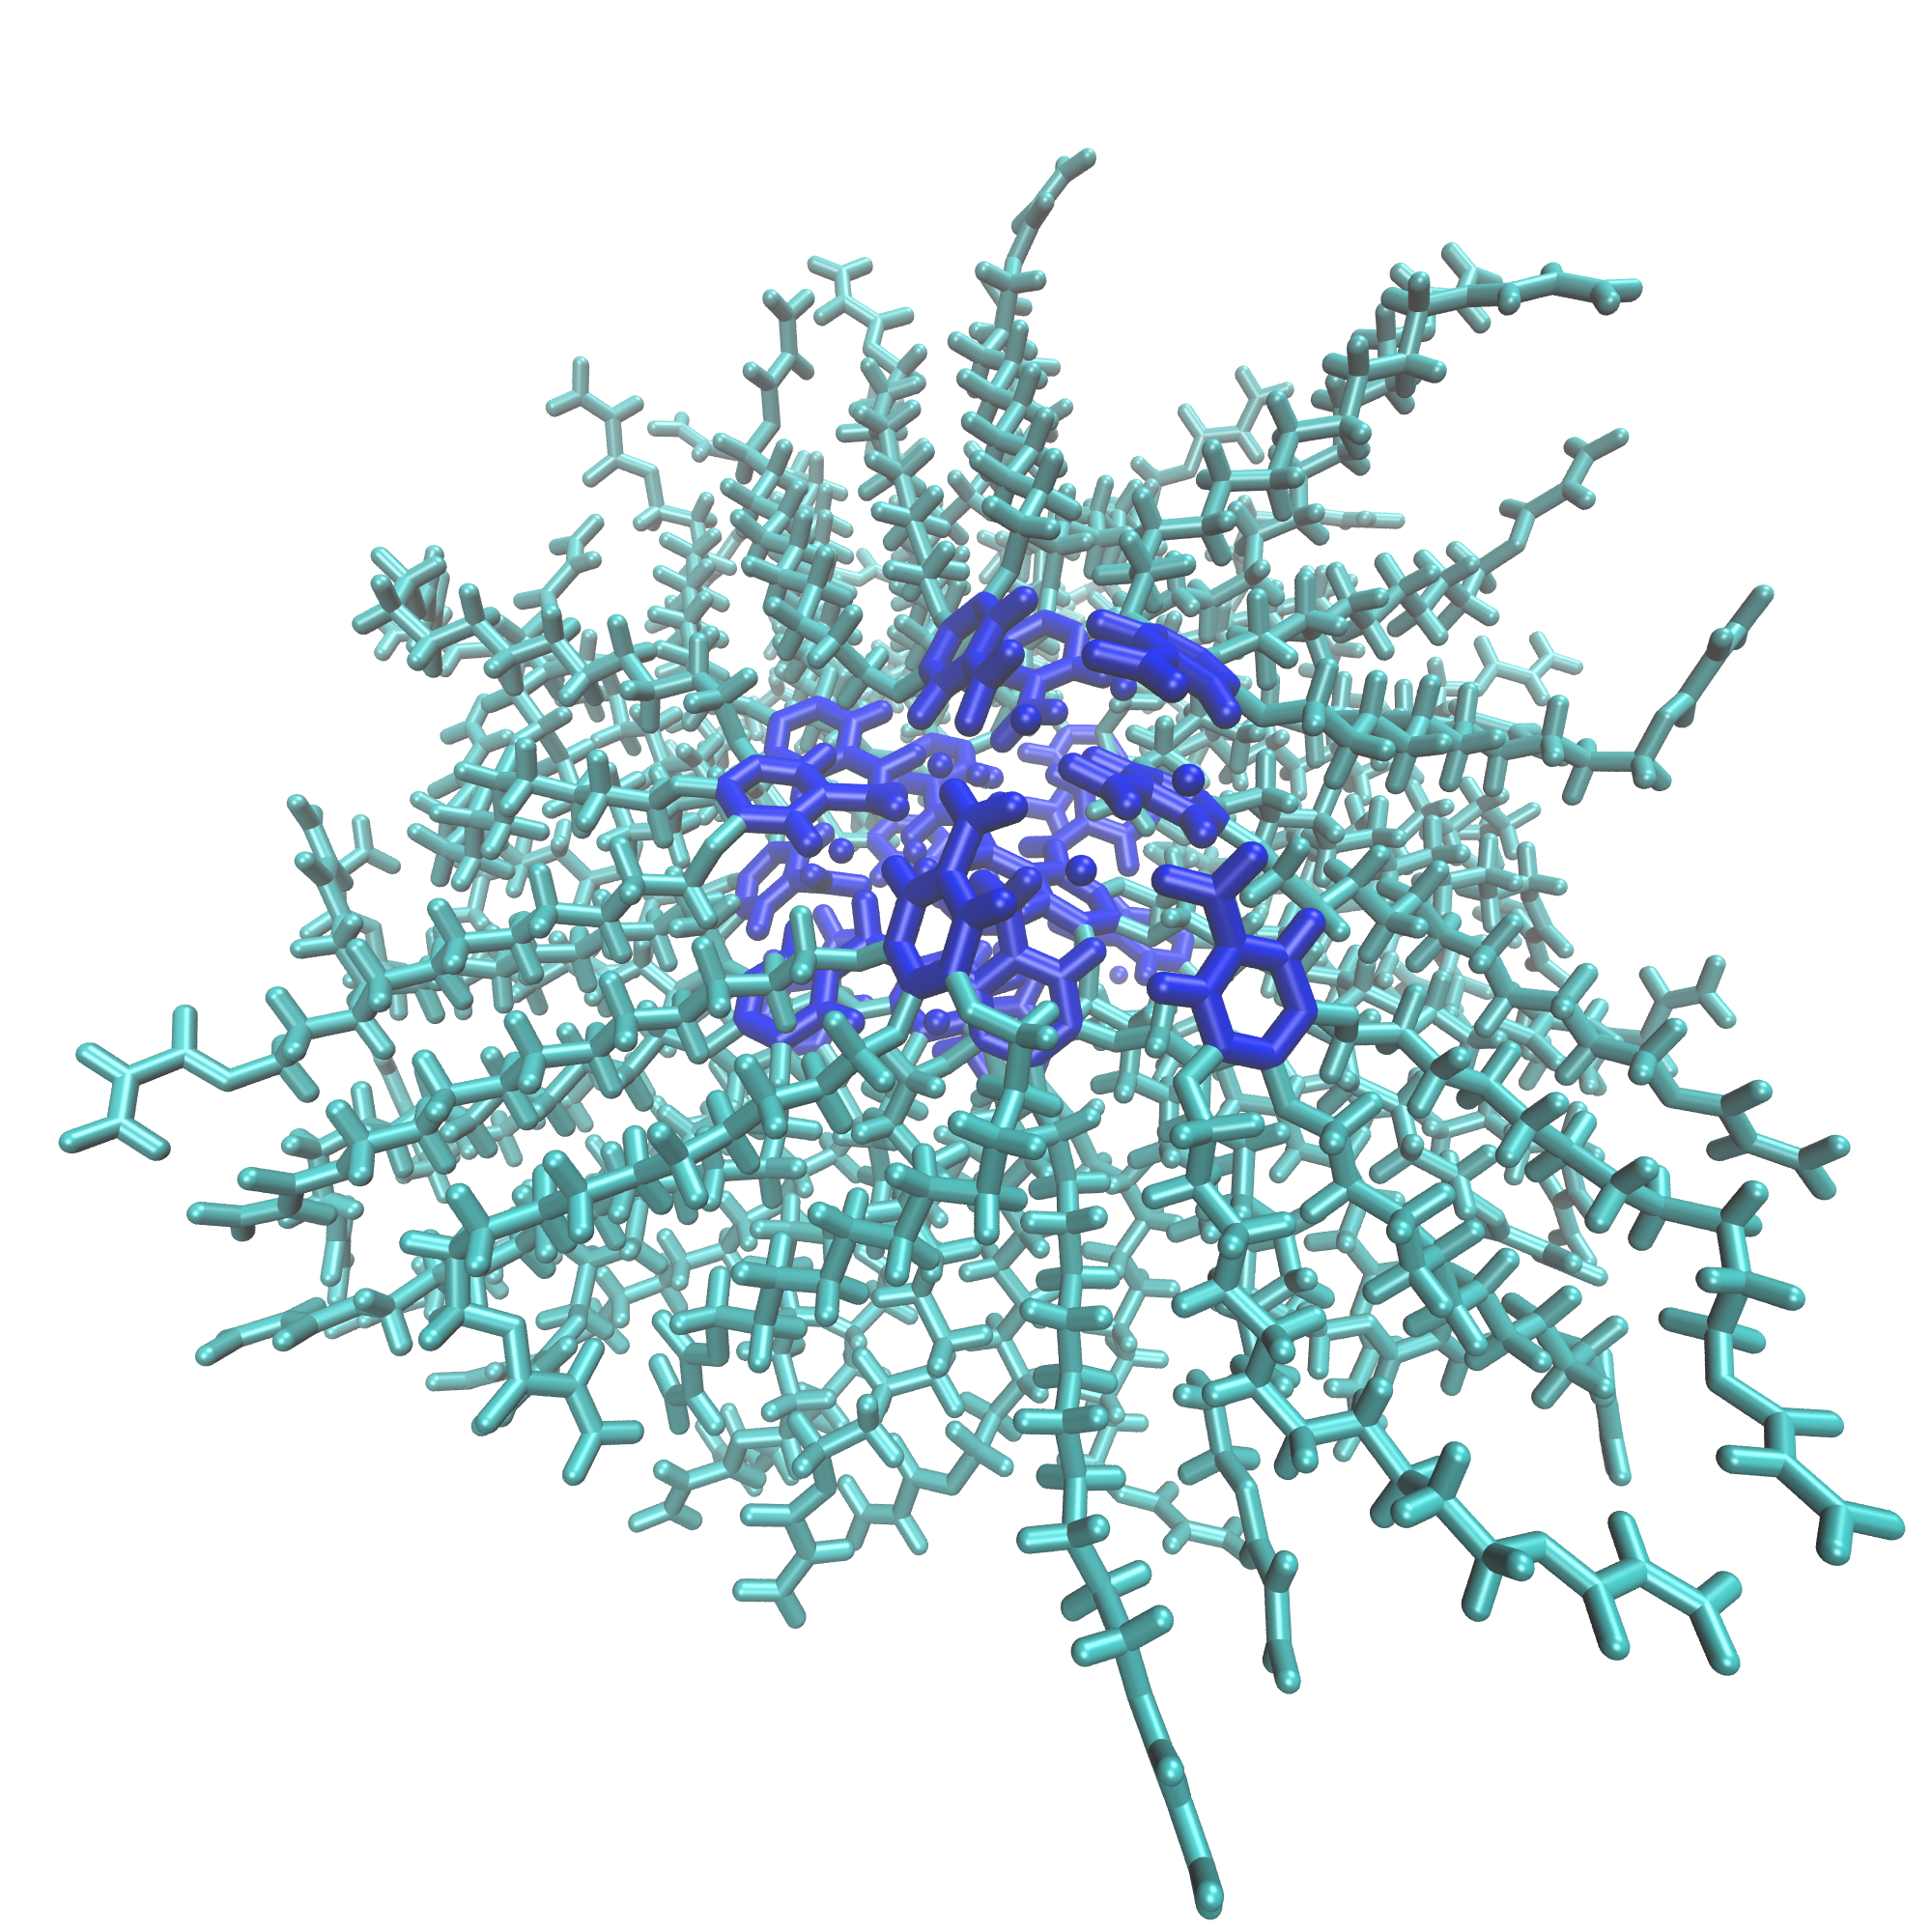
\includegraphics[width=\textwidth]{detailed_pore.png}
		\caption{}~\label{fig:detailed_pore}
	\end{subfigure}
%MRS6: this is one place where I might go to passive voice, since anyone can only speculate not just us.  
  \caption{We can only speculate about solute behavior inside the membrane
	  pores based on our previous picture of the pore structure (a). 
%MRS6: should be present text, not ``will use'' since it's what's happening in this paper. Look for this throughout.
          We will use a
	  detailed molecular model in order to appropriately model the pore's complex
	  architecture which is crucial to understanding the mechanism of solute
	  transport (b). The head group region is colored blue
%MRS6: probably mention from actual simulations we will describe below.
	  and the tail region is colored cyan in both representations.}~\label{fig:detail}
  \end{figure}
 
  Here we develop a model of the Col\textsubscript{h} assembly formed by
  Na-GA3C11. Compared to the H\textsubscript{II} phase, the Col\textsubscript{h}
  phase is a simpler starting point. The system has no water which will allow us
  to simulate longer timescales, and there exists detailed experimental
  characterization of the fully aligned state, including 2D wide-angle X-ray
  scattering (WAXS) patterns which are useful for reconstructing structural data.
  We anticipate using this Col\textsubscript{h} model in order to build an 
  H\textsubscript{II} model in the future.
  %The two phases appear to share similar structural characteristics since the
  %pore spacings in each system are in close agreement
  %\cite{feng_thin_2016,resel_structural_2000}.

  In order to appropriately model transport in these ordered, nanoporous
  organic systems, we must first gain a thorough understanding of the nanoscopic
  structure of LLC polymer membranes. Our current level of understanding about
  the structure at the nanoscale is limited. Using X-ray diffraction and TEM data
  we can infer that monomers aggregate into hexagonally packed columns with their
  head groups facing towards the column center. There remain several key questions
  that we will investigate in order to expand this understanding: 

  \begin{enumerate}

%MRS6: formatting suggestion
  \item \textit{If layers do exist, how many monomers constitute a single layer? \label{point:monomernum}} 
  A simple molecular simulation study of a similar molecule suggested that
  there are 4 monomers in each layer \cite{zhu_methacrylated_2006}. Their model
  likely does not sufficiently imitate the chemical environment present in the
  real system since it only contains 16 total monomers. A separate calculation
  for NA-GA3C11, based on the estimated volume of the liquid crystal monomers,
  proposes that each layer consists of seven
  monomers\cite{resel_structural_2000}. Our best chance to answer this question
  is by using a molecular model orders of magnitude larger than any other
  reported atomistic liquid crystal membrane simulation, as we present here. We
  will directly change the layer composition and note its effect on membrane
  structure.

  \item \textit{How do monomers in each layer position themselves with respect to
  surrounding layers? \label{point:orientation}}
  $\pi$-$\pi$ stacking interactions between aromatic monomer head groups may be
  a driving force of self-assembly in this system \cite{gazit_possible_2002}. Gas
  phase \textit{ab initio} studies of benzene dimers have shown a clear energetic
  advantage for parallel displaced and T-shaped $\pi$-$\pi$ stacking
  conformations over a sandwiched conformation \cite{sinnokrot_estimates_2002}.
  Substituted benzene rings exhibit an even stronger $\pi$-$\pi$ stacking
  attraction which favors the parallel displaced configuration in all cases
  except where the substitutions are extremely electron
  withdrawing\cite{waller_hybrid_2006,ringer_effect_2006}. In this study, we
  compare simulated X-ray diffraction patterns to experiment in order to deduce
  which stacking configuration is most likely. We also dive deeper into the
  origin of features present in the 2D diffraction patterns.  

  \item \textit{Does our model support the existence of layers and if so, how well
  defined are the layers? \label{point:layers}} 
  %BJC: Reordered, so changing the wording here.
  Indications of strong $\pi$-$\pi$ stacking interactions in the direction
  perpendicular to the membrane plane, combined with the wedge-like character of
  the LLC monomers, suggests that monomers should arrange into disks that stack in
  layers. $\pi$-$\pi$ stacking will only occur between the aromatic
  monomer head groups which leaves no description of what is happening in the
  monomer tail region. The tails may entangle isotropically while maintaining
  stacking order among headgroups. 

  \item \textit{Can the system exist in other metastable states or phases that are not
  accessed during experiments? \label{point:metastable}}
  There remains the possibility that there is more than one metastable state
  associated with a given LLC phase. Simulating a membrane atomistically
  requires many atoms which limits the timescales acessible with MD. It is
  reasonable to expect that we will generate configurations which are kinetically
  trapped in a metastable free energy basin. We must be able to identify which
  states 
  %MRS6: best not to set up too high expectations
  %is produced experimentally.
  are most consistent with experiment.

  \item \textit{What constitutes a pore, and what are the details of its pore architecture? \label{point:poredefinition}}
  The limited picture that experiment provides tells us that there are
  hexagonally packed, hydrophilic regions where transport is likely to occur.
  One may instinctively assume that these regions are hollow tube-like pathways.
  We will explore the composition of the pores and the partition between the
  hydrophilic and hydrophobic regions. 

  \item \textit{Is it necessary to include any water in order to appropriately model
  the Col\textsubscript{h} phase? \label{point:water}}
  While past work describes the Col\textsubscript{h} phase as dry~\cite{feng_scalable_2014}, 
  it has been suggested by experimentalists, in
  unpublished communications, that it is likely that neat monomer leaches small
  amounts of ambient water. Experimentally, achieving a hexagonal phase with a
  completely dry system has proven difficult. If neat monomer sits in ambient
  conditions, its color turns from transparent to slightly opaque and a hexagonal
  phase forms. Although we will not explore whether water is necessary for
  self-assembly, we hypothesize that the hydrogen bonding network formed by the
  water may play a role in structuring the pores and holding together the
  hexagonal phase. We can look at correlation functions and use simulated X-ray
  diffraction patterns to see if there is any meaningful structural difference
  between a ``dry'' and ``wet'' system.

  \end{enumerate}
  
  %Once we have addressed all of the above questions, we must show that the 
  %developed molecular model is consistent with physical observations so that we
  %can rely on conclusions drawn about structural features characteristic of 
  %the system.
 
  We used experimental small-angle X-ray scattering (SAXS) data from
  \cite{feng_thin_2016} (Fig.~\ref{fig:SAXS}) and wide angle X-ray scattering
  (WAXS) data (Fig.~\ref{fig:WAXS}, produced as described in
  \cite{feng_scalable_2014}) for comparison to our model. We rely primarily on the 2D WAXS data
  since it encodes all structural details down to the sub-nm scale.  There are
  five major features of interest present in the 2D experimental pattern shown in
  Figure \ref{fig:WAXS}.

  \begin{enumerate} 
  
	\item \textit{R-$\pi$}: The location of the first is at $q_z$ = 1.7
	\AA$^{-1}$, corresponding to a real space separation of 3.7 {\AA}. Previous
	work~\cite{feng_scalable_2014} attributes this reflection to $\pi$-$\pi$
	stacking between aromatic rings in the direction perpendicular to the membrane
	plane, or z-axis \cite{feng_scalable_2014}. For simplicity, we will refer to
	this reflection as R-$\pi$.
 
	\item \textit{R-helix}: A weak intensity line, located at exactly half
	the $q_z$ value of R-$\pi$ ($q_z$ = 0.85 \AA$^{-1}$), corresponds to a real
	space periodic spacing of 7.4 \AA~. This reflection has been interpreted as
	2\textsubscript{1} helical ordering of aromatic rings along the z axis
	\cite{feng_scalable_2014}, meaning that if one traces the positions of the
	aromatic rings with a helical curve, then for each full turn in the helix, one
	will encounter two aromatic rings. For this reason we will refer to reflection
	as R-helix. 

	\item \textit{R-alkanes}: A low intensity ring located at r = 1.4
	\AA$^{-1}$ marks the third major reflection of interest. The real space
	separation corresponds to 4.5 \AA~ which is characteristic of the average
	spacing between packed alkane chains \cite{mcintosh_organization_1980}. We will
	call this reflection R-alkanes.

	\item \textit{R-spots}: Within R-alkanes, are four spots of higher
	relative intensity.  Accordingly, we name these reflection R-spots. The
	location of all spots is $\sim\;37^{\circ}$ from the $q_z$ axis in their
	respective quadrants. In many liquid crystal systems one can explain the spots
	as the tilt angle of the alkane chains with respect to the membrane
	plane\cite{govind_simple_2001}.
 
	\item \textit{R-pores}: The final feature corresponds to the spacing
	and symmetry of the d\textsubscript{100} plane. This plane is geometrically
	related the distance between pores. The feature, which we named R-pores, is
	characterized by dots along the equatorial axis defined when $q_z$ = 0. The
	spacing between dots is indicative of the hexagonal symmetry of the packed
	pores. We observe the same information with higher resolution using SAXS
	(Fig.~\ref{fig:SAXS}). 

  \end{enumerate}

  \begin{figure}
        \centering
        \begin{subfigure}[t]{0.43\linewidth}
                \centering
                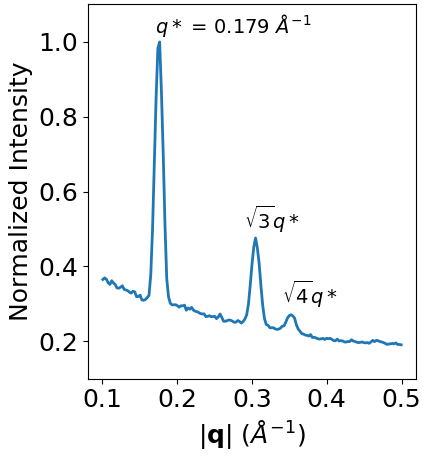
\includegraphics[width=\linewidth]{SAXS.png}
                \caption{}\label{fig:SAXS}
        \end{subfigure}
        \begin{subfigure}[t]{0.47\linewidth}
                \centering
                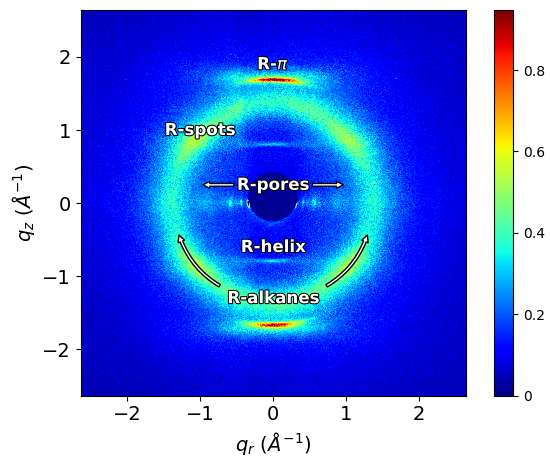
\includegraphics[width=\linewidth]{WAXS_annotated_words.png} 
                \caption{}\label{fig:WAXS}
        \end{subfigure}
%BJC: What do you think of the labels now? I tried to make it more clear what each label refers
% to graphically. I can't decide if it's too cluttered. An alternative is to number them as  
% I had them before, and then define them in a little box inset to the figure
	\caption{(a) (Reproduced from \cite{feng_thin_2016}) The repeat spacing
		in the 1D small angle X-ray scattering pattern is characteristic of hexagonal
		packing. The leading peak, q*, represents the distance between the
		d\textsubscript{100} planes. Using this distance, we know that the distance
		between pore centers is 4.12 nm. (b) 2D WAXS gives
		details about repeating features on the order of angstroms. Experimentalists
		have explained each of the 5 major reflections present as follows: (R-$\pi$) Aromatic
		head groups $\pi-\pi$ stack 3.7 \AA~apart. (R-helix) Monomers arrange vertically in
		a 2\textsubscript{1} helix. (R-alkanes) Alkane chain tails pack 4.5 \AA~apart. (R-spots)
		Monomer tails are tilted with respect to the membrane plane. (V) As derived from
		SAXS, the pores are spaced 4.12 nm apart and pack hexagonally}
	\label{fig:SWAXS}
 \end{figure}

  \section{Methods}
 
  \subsection{Monomer Parameterization}

  We parameterized the liquid crystal monomers using the Generalized AMBER
  Force Field \cite{wang_development_2004} with the Antechamber package
  \cite{wang_automatic_2006} provided with AmberTools16
  \cite{case_ambertools16_2016}. We assigned atomic charges using the am1bccsym
  method of \texttt{molcharge} shipped with QUACPAC from Openeye Scientific
  Software. We ran all molecular dynamics simulations using Gromacs 2016
  \cite{bekker_gromacs:_1993,berendsen_gromacs:_1995,van_der_spoel_gromacs:_2005,hess_gromacs_2008}.

  We generated an ensemble of characteristic, low-energy vacuum monomer
  configurations by applying a simulated annealing process to a
  parameterized monomer. We cooled monomers from 1000K to 50K over 10
  nanoseconds. We randomly pulled a low energy configuration from the
  trajectory then reassigned charges using \texttt{molcharge}. Using the new
  charges, we annealed the monomer system again and pulled a random monomer
  configuration from the trajectory which we used for full system
  construction (Figure~\ref{fig:python}a). See Supporting Information for
  further detail.

  \subsection{Unit Cell Preparation}

  The timescale for self-assembly of monomers into the hexagonal phase is
  unknown and likely outside of a reasonable length for an atomistic simulation,
  calling for a more efficient way to build the system. Previous work has shown
  a coarse-grained model self assemble into the H\textsubscript{II} phase
  configuration in $\sim$1000 ns \cite{mondal_self-assembly_2013}.  We
  attempted atomistic self-assembly by packing monomers into a box using Packmol
  \cite{martinez_packmol:_2009}. Simulations of greater than 100 ns show no
  indicators of progress towards an ordered system. To bypass the slow
  self-assembly process, we use Python scripts to assemble monomers into a
  structure close to one of a number of hypothesized equilibrium configurations
  (Figure~\ref{fig:python}).
  %MRS6: question; we would like to make these releasable in GitHub.
  %BJC2: yes .. what is the question?
  \begin{figure}
	\centering
	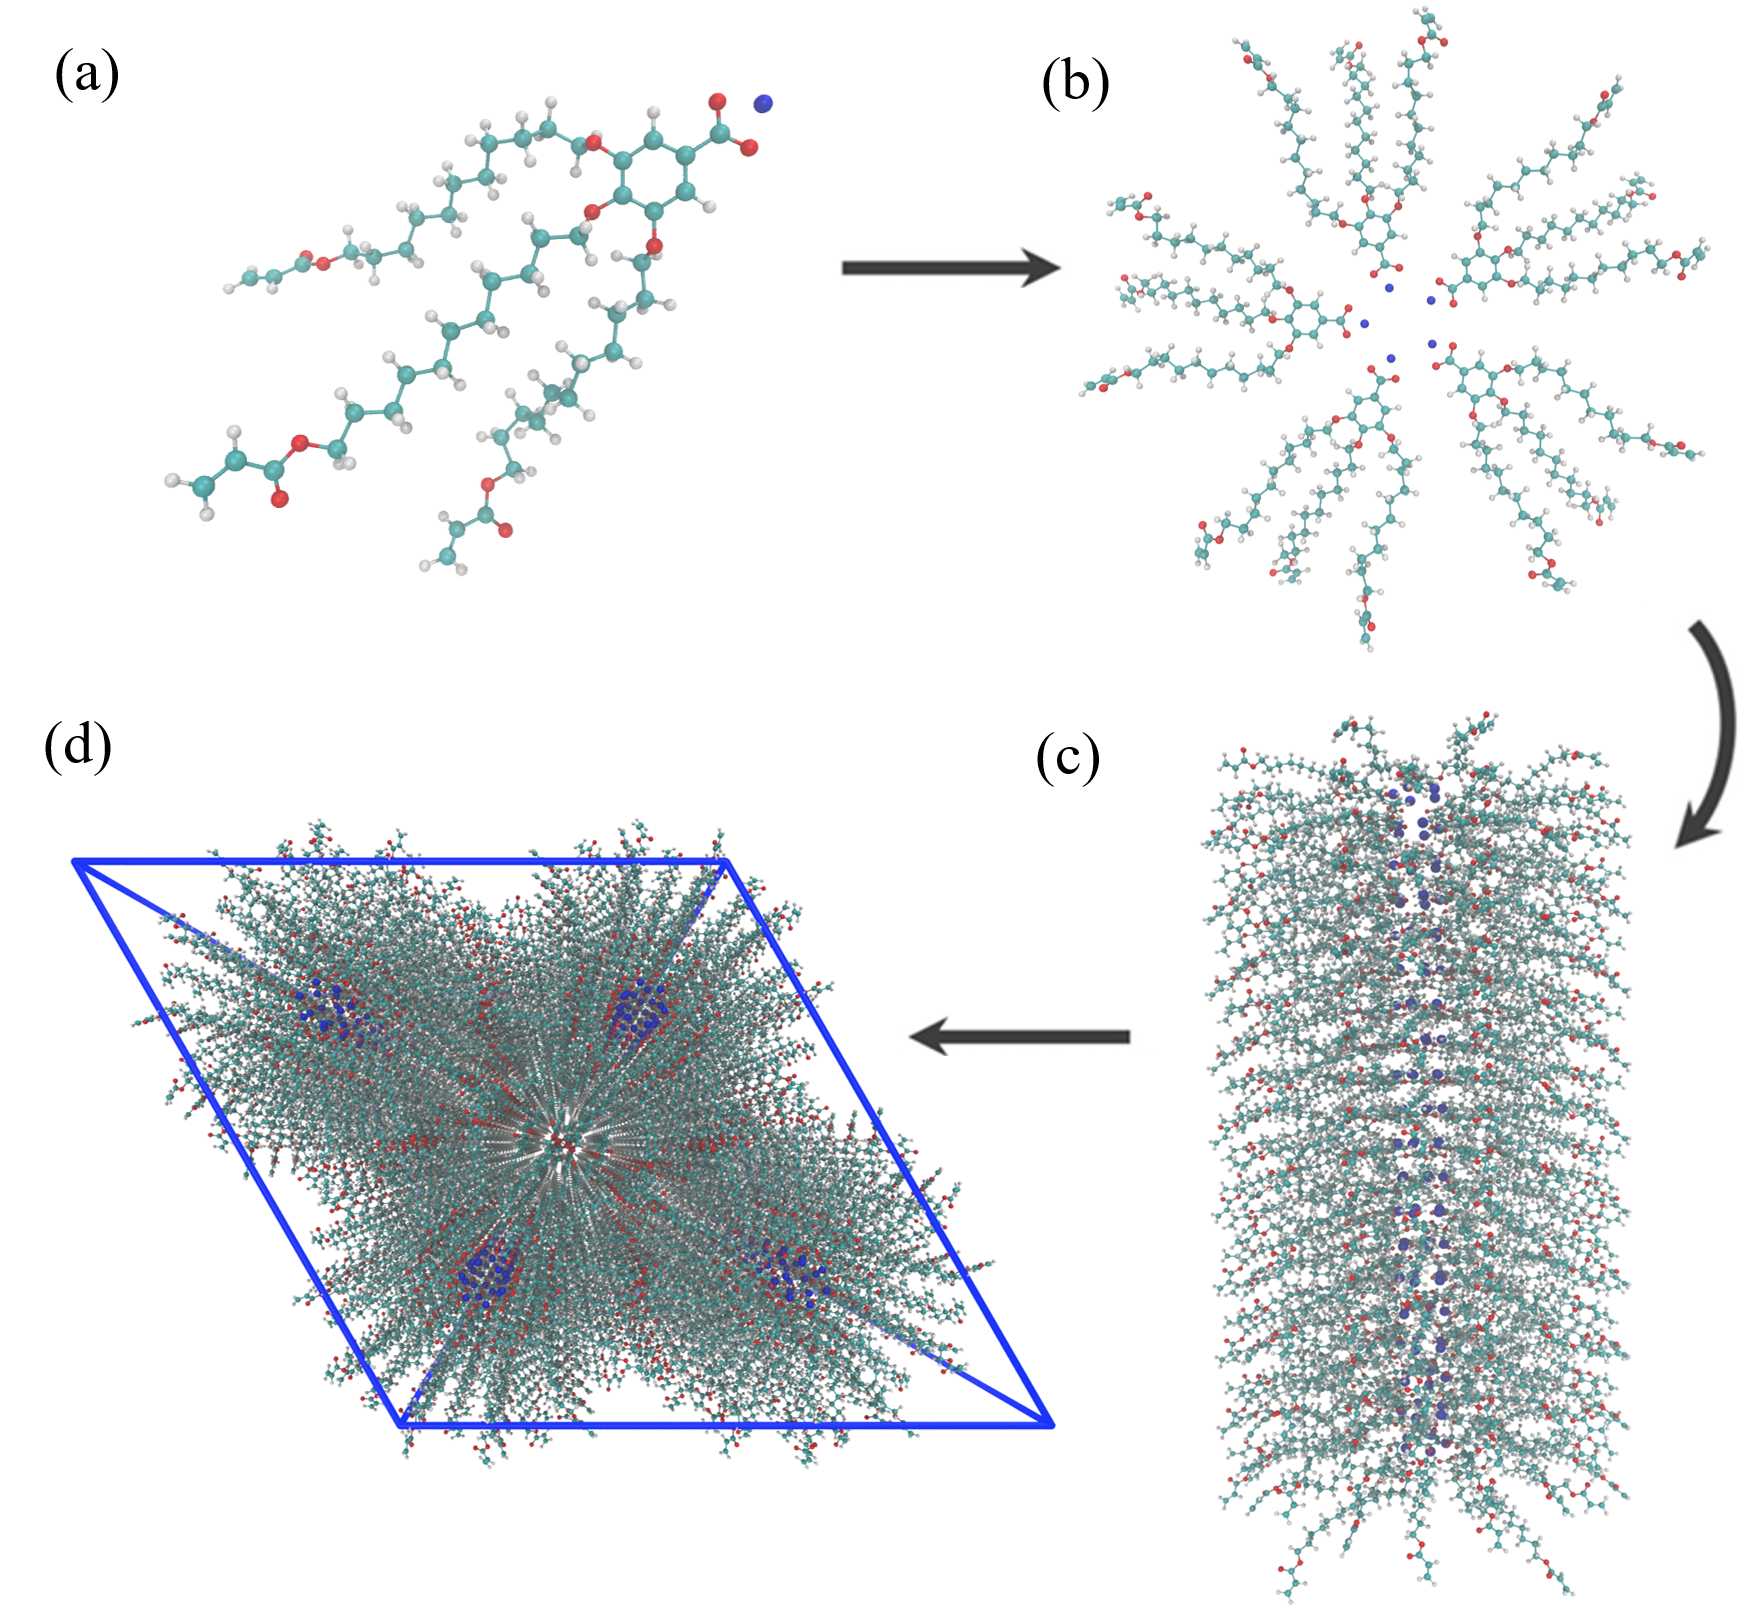
\includegraphics[width=0.75\linewidth]{build.PNG} %BJC: put an xyz axis with the unit cell
	\caption{(a) We parameterized a single monomer and annealed it to produce a low energy
		configuration. (b) A Python script rotates and assembles monomers into layers with 
		hydrophilic centers. (c) We chose to stack twenty layers on top of each other to create
		pores. (d) The pores are duplicated and placed into a monoclinic unit cell.}\label{fig:python}
  \end{figure}
  
  A typical simulation volume contains four pores in a monoclinic unit cell,
  the smallest unit cell that maintains hexagonal symmetry when extended
  periodically. Each pore is made of twenty stacked monomer layers with periodic
  continuity along the pore axis, avoiding any edge effects and creating an
  infinite length pore ideal for studying transport. We prefer a small number of layers
  in order to reduce computational cost and to allow us to look at
  longer timescales. Ultimately, we chose to build a system with 20 monomer
  layers in each pore in order to obtain sufficient resolution when simulating
  X-ray diffraction patterns. %This point will be explained in more detail later.
%MRS3: isn't there some observations you need at least 10?  
%BJC2: When I first set up the system, there was a gap and a small number of layers 
% appeared to cause the phase to disassociate. However, I can get a pretty small
% number of layers in the infinite pore system, but the diffraction is low resolution.

\subsection{Monomer Placement} 

  When constructing an initial configuration, there are a number of variables
  which require careful consideration while placing monomers. The equilibrium
  configuration is sensitive to some while insensitive to others. The starting
  pore radius, defined as the distance of a chosen head group carbon from the
  pore's central axis, does not influence the equilibrium structure if one choses
  a reasonable value. The pore radius is chosen to be 0.5 nm in our initial
  configurations. 
  %MRS6: added.
  The initial distance between pores, within a wide range, also has little effect on
  the the equilibrated structure. However, one should not start them too close or
  there will be high energy repulsions during early equilibration. We chose an
  initial pore spacing of 4.5 nm, $\sim$10\% larger than the experimental value
  of 4.12 nm.  A sensitivity analysis of both parameters is presented in
  the 
  %MRS6: check for J phys chem B to see if its supporting or supplemental information or material.
  %BJC2: good point. It is 'supporting information'
  Supporting information.  The distance between layers, the rotation of the
  layers with respect to adjacent layers, and the number of monomers per layer do
  influence the equilibrium structure and require further justification for their
  choices. We rely on experimental data to inform them. 

  We chose the layer spacing for the initial configuration based on R-$\pi$ and
  then allowed the system to readjust during equilibration. Each monomer was
  rotated so the plane of its aromatic head groups would be coplanar with the xy
  plane. We explored three different initial layer spacings. The first is exactly
  equal to R-$\pi$ with layers placed so aromatic rings stack 3.7 \AA~apart in
  the z-direction. We explore a second system with an initial layer spacing of 5
  \AA. We briefly explored a third system with an initial layer spacing of 10
  \AA, however it shows non-physical behavior which is detailed in the 
  Supporting Information. 

% This is true if initial equilibration is performed with pressure control
%  If we initially space layers too far apart, they will collapse on each
%  other while simultaneously slipping in between layers of adjacent pores, which
%  leads to an artificially thick membrane with pores spaced closely together.
%  Further details of simulations with layer stacked 10 \AA apart are in the supplemental
%  information.

  We chose the relative interlayer orientation based on clues from diffraction
  data as well as the various known stacking modes of benzene and substituted
  benzene rings: sandwiched, parallel-displaced and T-shaped
  \cite{sinnokrot_estimates_2002}. We ruled out the T-shaped configuration
  because its $\sim$5 \AA~equilibrium stacking distance
  \cite{sinnokrot_estimates_2002} is inconsistent with R-$\pi$. It is also
  infeasible for the monomers to orient in the T-shaped conformation because of
  the bulky tail groups. We will explore the system's preference towards the
  sandwiched vs. parallel displaced stacking modes in some detail. Both have
  reported stacking distances near the R-$\pi$ value of 3.7 \AA. Headgroups in
  our sandwiched initial configuration stack directly on top of each other while
  headgroups in the parallel displaced initial configuration stack with an offset
  of $180^\circ/nmon$ where $nmon$ is the number of monomers per layer. See
  the Supporting Information for a detailed illustration of the initial
  configurations in each mode.

  The number of monomers in each layer is unknown, as stated in question
  (\ref{point:monomernum}). We tested configurations constructed with a varied
  number of monomers per layer. We built systems in the offset and parallel
  displaced configurations with 4, 5, 6, 7 and 8 monomers per layer.

  \subsection{Equilibration}

  We developed equilibration schemes to create dry and wet configurations. Both
  schemes start with an initial configuration generated according to the previous
  guidelines. To create a dry configuration, we fix monomer head groups in the
  sandwiched or parallel-displaced configuration using position restraints with a
  force constant of 10$^6$ kJ mol$^{-1}$ nm$^{-2}$. We run a 50 ps simulation in
  the NVT ensemble which allows the monomer tails to settle without disrupting
  the ordering of the head groups. Doing so also mitigates system dependence on
  initial monomer configuration. Every 50 ps, we reduce the force constants by
  the square root of its previous value. Once the force constant is below 10 KJ
  mol$^{-1}$ nm$^{-2}$, we reduce the restraints in a sequence with values of
  8, 3, 2, 1, and 0 KJ mol$^{-1}$ nm$^{-2}$ respectively. We allow the resulting
  unrestrained structure to equilibrate for 5 ns in the NPT ensemble
  with pressure controlled by the berendsen barostat. Next, we run long NPT
  equilibration simulations for at least 400 ns using the Parrinello-Rahman
  barostat with a time constant of 10 ps.

  %MRS6: some parameters missing here (time run between insertions, etc). 
  %I assume they are in supporting information?
  %BJC2: Not there yet but will add
  In order to create a ``wet'' system, we solvated an initial configuration with
  water using \texttt{gmx solvate}. We remove all water molecules placed outside
  the pore region. Then we randomly remove water molecules inside the pore region
  until the pores reach the desired concentration of water. The remainder of the
  equilibration follows the same procedure as the dry system. 

  \subsection{Cross-linking}
  
  In order to fully match synthetic procedures, we created a cross-linking
  algorithm that one can apply to equilibrated structures. The purpose of
  cross-linking is to maintain macroscopic alignment of the crystalline domains,
  ensuring aligned, hexagonally packed pores. For that reason, we are not
  concerned with replicating the kinetics of the reaction, but instead emphasize
  the consistency of the final structure with experimental structural data. 

  We developed the algorithm based on the known reaction mechanism.
  Cross-linking of this system is a free radical polymerization (FRP) taking
  place between terminal vinyl groups present on each of the three monomer tails.
  FRPs require an initiator which bonds to the system, meaning new atoms are
  introduced into the system. For simplicity, we simulated the initiator as
  hydrogen and made it present in the simulation by including them as dummy atoms
  in all possible locations where an addition could occur. We carry out the
  cross-linking procedure iteratively. During each iteration, the algorithm
  selects eligible bonding carbon atoms based on a distance cut-off. The topology
  is updated with new bonds and dummy hydrogen atoms are changed to appropriate
  hydrogen types.  Head-to-tail addition was the only propagation mode considered
  due to its dominance in the real system \cite{young_introduction_2011}. We did
  not consider direction of attack because the resultant mixture is racemic.

  Our implementation requires long simulation times to achieve high cross-link 
  densities. A typical cross-linking procedure can take up to 24 hours. In
  order to collect equilibrated data, further NPT simulation is necessary. We
  typically run a cross-linked system for an additional 100 ns to allow the system
  to readjust. For those reasons we did not cross-link all systems tested, but only
  the most promising structure. We show that cross-linking does not significantly
  change any of our drawn conclusions in Section 3.6.

  \subsection{Equilibrium Calculations}

  \subsubsection{\textit{Determining equilibration time}}

  Using equilibrated structures, we carry out various calculations to
  characterize the system. We define the point at which a system is equilibrated
  based on when the distance between pores stops changing.  We determined when
  the distances stopped changing by applying the statistical test,
  \texttt{pymbar.timeseries.detectEquilibration}, to the time series
  \cite{chodera_simple_2016,shirts_statistically_2008}. Simulations of 400 ns
  give at least 50 ns of equilibrated simulation trajectory.

  \subsubsection{\textit{Calculation of pore spacing}}

  To calculate the equilibrated pore spacing, we measured the distance between
  pore centers. We located the pore centers by averaging the coordinates of sodium
  ions in their respective pores. We generated pore spacing statistics 
  using the bootstrapping technique (See Supporting Information).

  \subsubsection{\textit{The nematic order parameter}}

  We calculated the nematic order parameter for our system in order to
  understand the degree of ordering among monomer head groups. Typically, the
  nematic order parameter is calculated for nematic liquid crystal systems which
  are characterized by unidirectional ordering of liquid crystal monomers. The
  preferred direction of monomers is defined by the unit director vector,
  $\mathbf{n}$. Assuming a single preferred direction of alignment, the nematic
  order parameter, $S$, is defined as:
  \begin{equation}
	 S = \frac{1}{2} \langle(3\cos^2\theta -1)\rangle
	\label{eqn:nematic_order_parameter}
  \end{equation}
  where $\theta$ is the angle between the molecular long axis and $\mathbf{n}$.
  In a perfectly ordered system, the molecular axis should be aligned with
  $\mathbf{n}$ and give an order parameter of $S=1$. We are interested in
  quantifying the degree of monomer head group alignment between systems. We use
  Eq.~\ref{eqn:nematic_order_parameter} to accomplish this by defining
  $\mathbf{n}$ as the z-axis (or pore axis), and then measuring the angles,
  $\theta$, between $\mathbf{n}$ and the vectors perpendicular to the plane of
  the aromatic head groups. See the Supporting Information for a diagram.  
  
  \subsubsection{\textit{Pair distribution functions}}

  The normalized pair distribution function, $g(\mathbf{r})$, describes
  the probability of finding a pair of particles separated by $\mathbf{r}$,
  \begin{equation}
	g(\mathbf{r})= \frac{1}{\rho N} \Bigg \langle \sum_{i=1}^{N}\sum_{j\neq i}^{N} \delta(\mathbf{r}+\mathbf{r_j}-\mathbf{r_i}) \Bigg \rangle
	\label{eqn:correlation}
  \end{equation}
  where $\rho$ is the average number density of particles and
  $\delta(\mathbf{r})$ is the Dirac delta function\cite{kuriabova_linear_2010}.
  We applied equation \ref{eqn:correlation} in three dimensions and then
  extracted one and two dimensional distribution functions by collapsing the grid
  along the appropropriate axes.

  In the 1D case, we measured the pair distribution function between centers of
  masses of aromatic head group rings, $g(z)$, along the z-axis (perpendicular to
  the membrane plane). To extract the average distance between layers we applied
  a discrete Fourier transform to $g(z)$ and extracted the highest intensity
  frequency. We performed the same procedure to calculate $g(z)$ of the tails 
  except instead of using the center of masses of the tails, we averaged $g(z)$
  for each atom that makes up the tail.

  In two dimensions, we observed xy and xz pair distribution functions based on
  the center of masses of the aromatic head group rings. For the xy pair
  distribution functions, we used a rotated frame of reference. For a given center
  of mass, we rotated the coordinates so that the vector created from the center
  of mass to the pore center was aligned with the positive x-axis. 

  %We gave special
  %consideration to the xy cross-sections since multiple rings exist in the same
  %plane located at different vertices of a polygon. We used a rotated frame of
  %reference to avoid ambiguity in the final pair distribution functions. i


  \subsubsection{\textit{Radial distribution functions}}
  Closely related to the spatial correlation functions, we explored the pores'
  compositions by measuring the average number densities of various monomer
  components as a function of distance from the pore centers. We looked at the
  average number density of sodium ions, aromatic rings and carbon atoms making
  up the monomer tails. We binned the radial distance of all atoms in each group
  from the pore centers, then normalized by the volume of the annulus defined by
  the bin edges and the z box vector (See Supporting Information for a 
  diagram). 

  \subsubsection{\textit{Simulated structure factor calculations}}
  % BJC: To be replaced by Joe's description
  {\color{red}This section replaced by Yelk/Glaser text}. 
  Simulated X-ray diffraction patterns are generated based on atomic
  coordinates in order to make a direct experimental comparison. All atomic
  coordinates were simulated as Gaussian spheres of electron density
  corresponding to each atom's atomic number. A three dimensional Fourier
  transform (FT) of the array of electron density results in a three dimensional
  structure factor which represents the unit cell in reciprocal space. We matched
  experimental 2D WAXS patterns by adjusting the initial spacing between layers
  and the orientation of the head groups with respect to adjacent layers.

  We normalized the colorbars on all diffraction patterns relative to
  R-alkanes. We believe that the alkane-alkane density, averaged over all angles,
  is the feature most likely to be replicated between experiment and simulation.
  Other features are dependent on system ordering which is likely to have some
  dependence on initial configuration. We calculated the average intensity within
  R-alkanes of the experimental pattern, $I_{avg}$. We exclude intensities within
  $\pm$ 30\degree~of the meridional axis defined by $q_r=0$ , since the simulated
  patterns differ from experiment in those regions in all cases. Specifically, in
  contrast to the experimental WAXS pattern, R-$\pi$ appearing in simulated
  diffraction patterns intersects with R-alkanes (See Fig. \ref{fig:XRDsim}). We
  multiplied $I_{avg}$ by a scaling factor, $f$. Intensities that appear in the
  experimental pattern $\geq$ $f\times I_{avg}$ are colored uniformly. We apply
  the same scaling method to the simulated patterns. We carefully chose a scaling
  factor of $f=3.1$ in order to (1) visibly display all features in the
  experimental pattern and (2) to allow us to compare the relative intensities of
  features between simulated and experimental diffraction patterns.

  \subsubsection{\textit{Ionic conductivity calculations}}

  We calculated ionic conductivity using two different methods for robustness.
  The Nernst-Einstein relation, relates the DC ionic conductivity, $\sigma$, to ion
  diffusivity, $D$, concentration, $C$, ion charge, $q$, the Boltzmann constant,
  $k_b$, and temperature, $T$: 
  \begin{equation}
	\sigma = \dfrac{q^2CD}{k_b T} 
	\label{eqn:nernst_einstein}
  \end{equation}
  We measured sodium ion diffusion coefficients by calculating the slope
  of the linear region of the z-direction mean square displacement curve as
  indicated by the Einstein relation \cite{einstein_investigations_1956}. We
  visualized the MSD plot to determine where to begin and end a linear fit. We
  measured ion concentration with respect to the volume of the entire unit cell. 
  The second method, termed the Collective Diffusion model, measures the
  movement of the collective variable, Q, which is defined as the amount of
  charge transfer through the system and can be thought to represent the center
  of charge of the system. The conductance, $\gamma$, of the system can be
  calculated as:
  \begin{equation}
	 \gamma = \dfrac{D_Q}{k_b T} 
	\label{eqn:collective_diffusion}
  \end{equation}
  We convert the resulting value to ionic conductivity by multiplying by
  channel length and dividing by the membrane cross sectional area. $D_Q$ is the
  diffusion coefficient of the collective variable Q. It is calculated using the
  Einstein relation. One can access a detailed derivation of the model elsewhere
  \cite{liu_collective_2013}.

  \section{Results and Discussion}
  
  \subsection{Structural Characterization}
  
  \subsubsection{Number of monomer per layer}

  Our simulations best support a model built with 5 monomers per layer based on
  the measured equilibrated pore-to-pore distances. To discern the composition of
  the monomer layers, addressing question (\ref{point:monomernum}), we ran
  simulations of systems created with 4--8 monomers per layer. We built systems
  in both the parallel displaced and sandwiched configurations with layers
  initially spaced 3.7 \AA~apart. We prepared equilibrated configurations
  according to the dry equilibration procedure. All systems are stable after 400
  ns of simulation. 
  %MRS6: Above, probably need to be a bit more clear what you mean by stable (no noticable drift in pore-to-pore), and if you are only using data after the point of stability.
  %BJC2: I believe this is included in methods. I can restate if that's not clear
In a sense, all systems are at least metastable, addressing
  question (\ref{point:metastable}), however not all will make physical sense or fit
  the experimental profile that we are trying to match. Figure~\ref{fig:p2p}
  shows 
%MRS6:
%the pore spacing 
the equilibrated pore-to-pore distances 
for all systems tested. 
Systems built with 5 monomers in
  each layer equilibrate to a pore spacing that is most consistent with the
  experimental value of 4.12 nm derived from SAXS measurements
  (Figure~\ref{fig:SAXS}). 
%MRS6: discuss very briefly how far off 4 and 6 are to motivate selecting 5 exclusively.
The remainder of this discussion will focus on the
  analysis of systems built with 5 monomers per layer.

  \begin{figure}
	\centering
	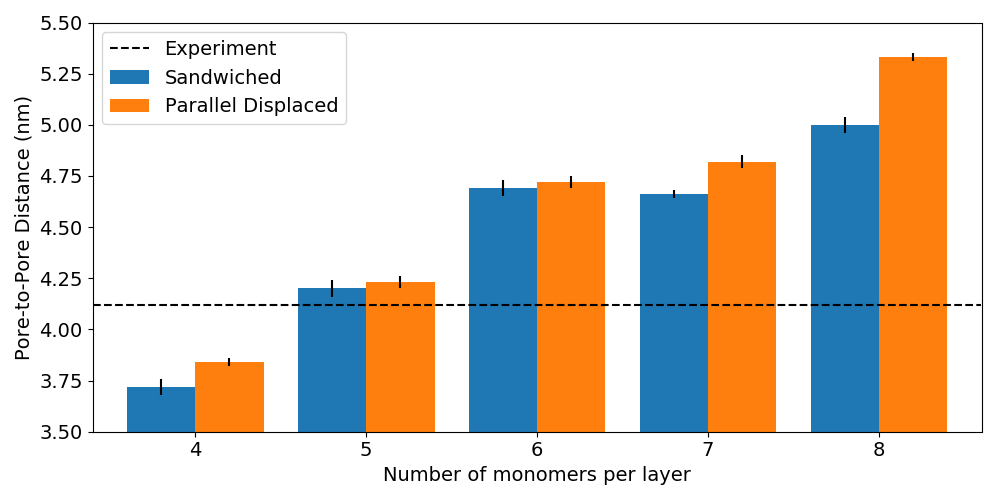
\includegraphics[width=\linewidth]{p2p.png}
        %MRS6: should there be a grapical demonstration of sandwiched vs. parallel displaced, especially equilbrated?
        %MRS6: some tweaks below.
	\caption{Systems with 5 monomers per layer have
		equilibrated pore spacing closest to the experimental value of 4.12 nm. The
			equilibrated pore spacing of the model increases as the number of monomers in
			each layer increases. The pore spacing of systems starting in the sandwiched
			configuration is systematically lower than those started in the parallel
			displaced configuration.}~\label{fig:p2p}
  \end{figure}  

  \subsubsection{Relative interlayer head group orientation}

  We answer question (\ref{point:orientation}) by simulating X-ray diffraction
  patterns produced from equilibrated MD trajectories. We tested systems built
  with 5 monomers per layer in the parallel displaced and sandwiched
  configurations. We generated simulated patterns using portions of simulation
  trajectory after equilibration. The patterns for both structures are shown and
  compared to experiment in Figure \ref{fig:XRDsim}.

  Simulated XRD of the sandwiched configuration contains all experimental
  features except for R-helix. R-alkanes, R-spots and R-pores appear close to their
  expected locations. R-$\pi$ is also present, however it intersects R-alkanes at
  a $q_z$ value lower than experiment meaning the head groups in our model prefer 
  to stack farther apart. 

  The parallel displaced configuration results in a simulated XRD pattern with
  the closest match to experiment. It produces the only pattern that exhibits all
  major reflections. R-alkanes and R-pores appear as they do in the sandwiched
  configuration. R-spots and R-$\pi$ appear, however with a lower intensity
  relative to R-alkanes when compared to the sandwiched configuration. R-helix
  appears due to the parallel displaced aromatic rings. It is a subharmonic of
  R-$\pi$ since the nearest vertically stacked head group to any given head group
  is $2\times$R-$\pi$~away. 
  %BJC: adjust figure size and alignment -- probably easiest to set figure size in matplotlib
  \begin{figure}
  \begin{subfigure}{0.3\linewidth}
        \centering
        \vspace{-0.2em}
        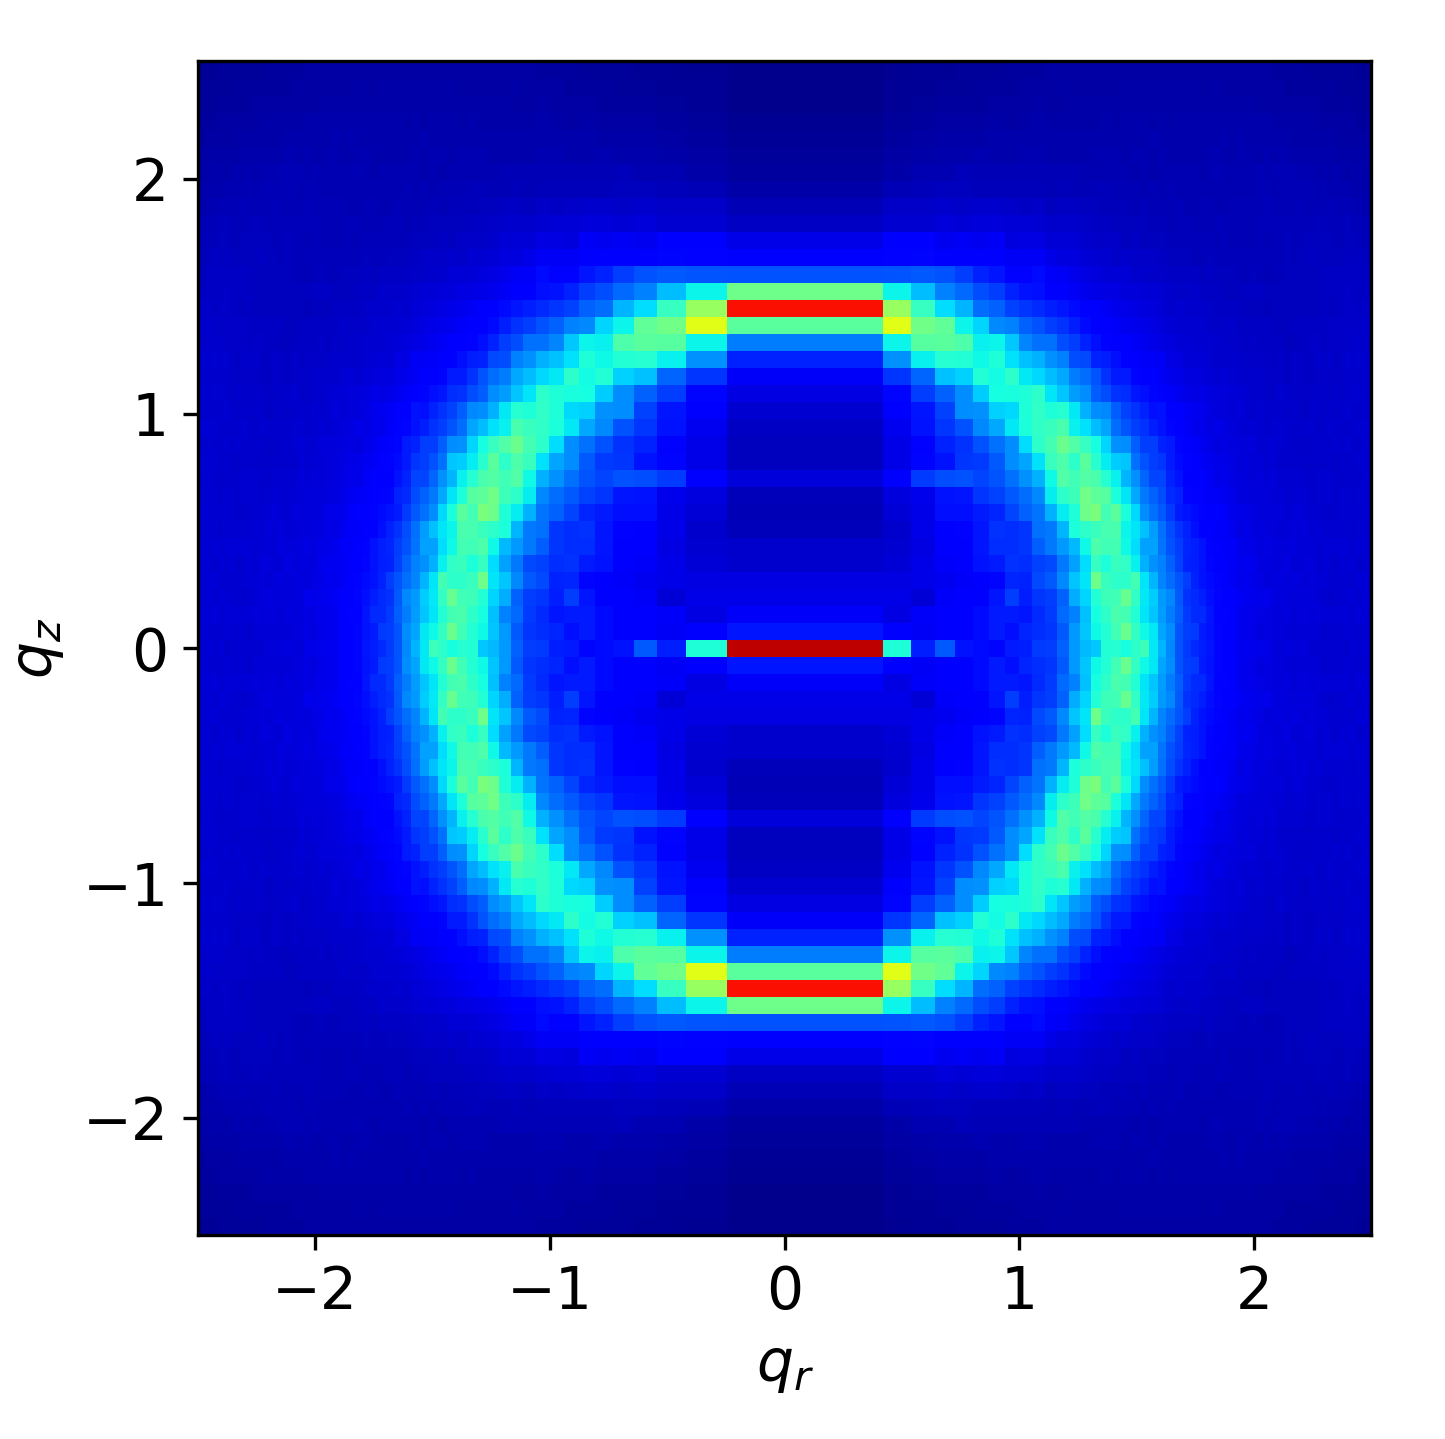
\includegraphics[width=1.1\linewidth,trim={1cm 0 1.3cm 0},clip]{offset_rzplot.png}
        \caption{}~\label{fig:rz_offset}
  \end{subfigure}
  \begin{subfigure}{0.3\linewidth}
        \centering
%        \vspace{0.25em}
        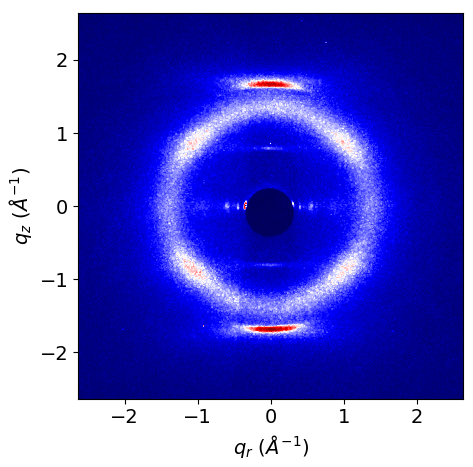
\includegraphics[scale=0.285]{WAXS_raw.png}
        \caption{}~\label{fig:raw_waxs}
  \end{subfigure}
  \begin{subfigure}{0.3\linewidth}
        \centering
        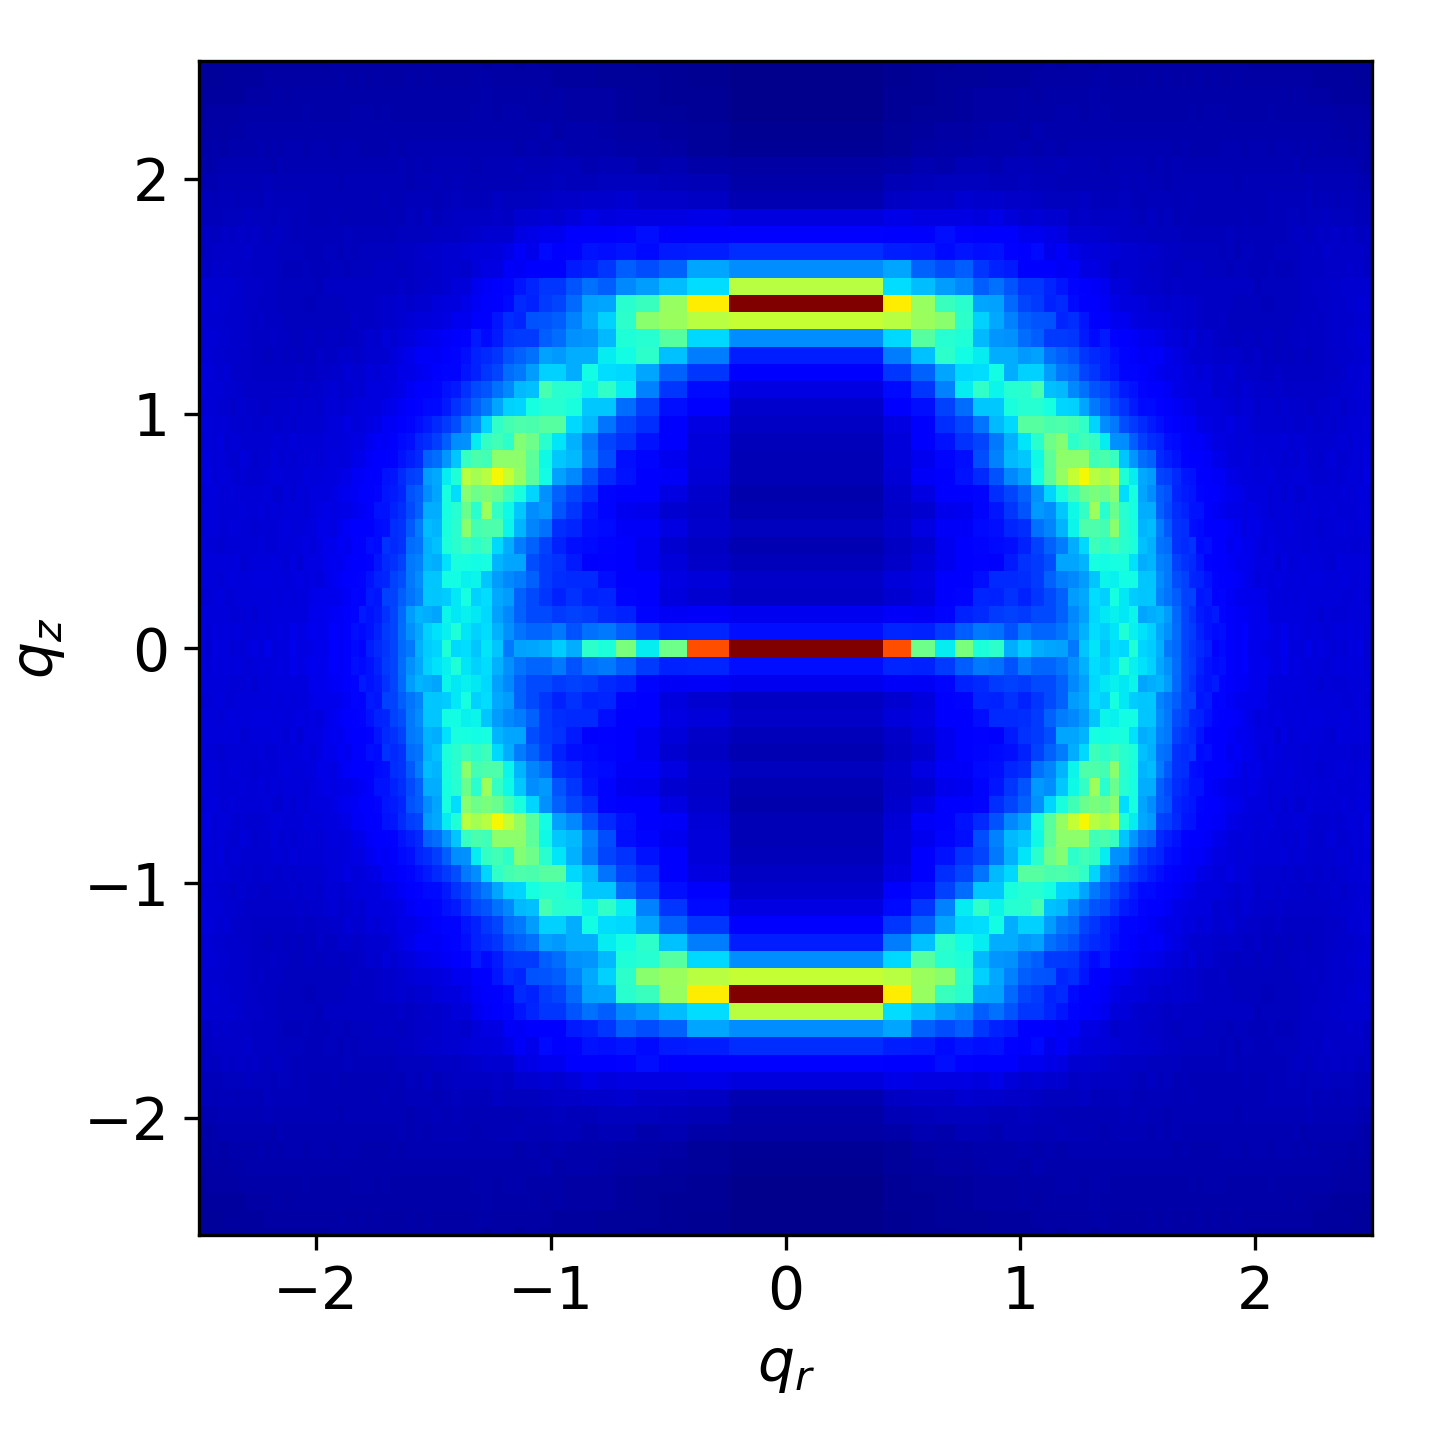
\includegraphics[width=1.1\linewidth,trim={1cm 0 1.3cm 0},clip]{layered_rzplot.png}
        \caption{}~\label{fig:rz_layered}
  \end{subfigure}
  \begin{subfigure}{0.0544\linewidth}
        \centering
        \vspace{-4.00em}
        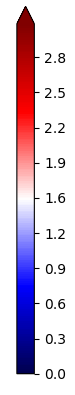
\includegraphics[width=\linewidth]{colorbar_seismic.png}
  \end{subfigure}
%MRS6: question: the SAXS region looks different between sandwiched and parallel displaced. Any thoughts why? We can discuss in person.  And seems like have to comment on the difference in intensity between Sandwich and parallel displaced in the pi-pi region.
%MRS6: I wonder to what extent showing the reflections of tails removed would make it clearer pi-pi is really there.  Maybe in supporting info?
%BJC2: Sure, I'll add that to supporting info
  \caption{The simulated XRD pattern generated from the equilibrated trajectory
	  of the parallel displaced configuration (a) exhibits all major reflections
	  present in the experimental WAXS pattern (b). The simulated XRD pattern
	  generated from the equilibrated trajectory in the sandwiched configuration (c) shows
	  all major reflections except R-helix.}
  \label{fig:XRDsim}
  \end{figure}

%  In both simulated diffraction patterns R-alkanes appears in the expected location. 
%  The location of R-pores is not well-defined in comparison to experiment. In order
%  to resolve those reflections it would be necessary to simulate a much larger system, 
%  but that is unnecessary since we can measure pore spacing manually as described 
%  earlier. R-$\pi$ and R

  In both the parallel displaced and sandwiched configurations, we noted that
  R-$\pi$ appears in a location which corresponds to a real space separation
  larger than experiment. We attribute this discrepancy to GAFF's inability to
  appropriately model the aromatic interactions which would be necessary to
  achieve the correct $\pi$-$\pi$ stacking distance. 
  %Systems have been modeled that exhibit the correct stacking distance, however
  %they are typically made of planar molecules spanning a large area.
  %BJC: I saw a paper like this a long time ago, but failed to save the citation and
  % now I am having a hard time finding it again. 
  The monomers in our model have bulky tails whose entropic contributions compete
  with the $\pi$-$\pi$ stacking interaction energy. There have been efforts to
  model systems that contain $\pi$ interactions in a classical mechanical context
  using polarizable forcefields \cite{baker_polarizable_2015},
  %MRS6: 
  but they are significantly more computationally expensive to
  reach the time scales required to equilibrate these systems at the present time.
  %MRS6: not so relevant below.
  %We could
  %implement a polarizable force field, however it is likely not worth the extra
  %computational cost. If our model proves to be inadequate when simulating
  %transport, we will revisit our current choice of forcefield.  

  In addition to R-$\pi$ being shifted to lower $\mathbf{q}$ values, a few
  factors combine to make the simulated R-$\pi$ reflection visibly more intense
  than in the experimental pattern. The simplest reason is that R-$\pi$ and
  R-alkanes add together to boost the overall signal at interesecting values of
  $\mathbf{q}$. In addition, we observe a much higher maximum intensity within
  R-$\pi$. The maximum intensity within R-$\pi$ of the normalized experimental
  pattern is 3.1, while the maximum intensity within R-$\pi$ of the normalized
  parallel displaced simulated pattern is 32.9. 
  %MRS2 10x is really big.  That seems hard to actually manage . . . I didn't realize it was that big. For some reason, I thought it was around 3x.  If it's that big, how come the 7.4 A reflection isn't big?  It's not clear to me how this is possible. Not clear how the angle averaging obscured this before?
  %BJC2 From plots of raw structure factor, it doesn't seem like a normalization issue. It was probably obscured in the orginal angle averaging because it 
  % was averaged with neighboring bins
  While direct numerical
  comparisons between simulation and experiment aren't necessarily precise due to
  underlying assumptions, an order of magnitude difference suggests some
  significance. We believe that we see such a high maximum for two reasons: (1)
  We are simulating a perfectly aligned system so all X-rays reflected along the
  pore axis would add constructively. The crystalline domains in the real system
  are not perfectly aligned (See azimuthal distribution in Supporting
  Information) which would lead to an overall decrease in the intensity of
  R-$\pi$. (2) Our system is more ordered with high correlation between layers.
  We will come back to this point further in ensuing discussions.

  There is a grid-like pattern near $\mathbf{q}=0$ which appears because the
  simulated system shows crystalline character. The grid features along nonzero
  values of $q_z$ line up with reflections at $q_z=0$ which indicates positional
  correlations between columns in the z-direction. This type of correlation is
  expected for a crystalline material. 
%MRS6: need some justification for why we are not totally surprised the system is crystalline.  But is is so crystalline in the x direction? The grid spacing is ``crystalline-ish'' in both x and z directions. . . we should talk. 
If our system met the definition of a
  columnar liquid crystalline system, we should observe only weak short-range
  z-directional correlation within columns, with no correlation between
  columns\cite{chaikin_principles_1995}. 

  The R-spots signal, which appears in both simulated XRD patterns, is not a
  result of alkane chain tilt. Previous literature has attributed the spots in
  this particular WAXS pattern as the product of tilted alkane
  chains~\cite{feng_scalable_2014}. We looked closer at the sandwiched
  configuration since R-spots appears with the most strength in its simulated XRD
  pattern. We measured the tilt angle of the alkane chains and showed that our
  system equilibrates to an average tilt angle close to zero degrees
  (Fig.~\ref{fig:tilt}). To understand the origin of R-spots, we determined which
  atoms gave rise to the feature. Since R-spots is present as higher intensity
  spots within R-alkanes, it is likely that the spots arise as a consequence of
  the tails. By removing all non-tail atoms from the trajectory and simulating a
  diffraction pattern, we were able to isolate the cause of the spots to the
  tails (Figure~\ref{fig:tails}). Since the tails stay nearly flat, we plotted
  the centroids of the tails and measured the angle between each centroid and its
  nearest neighbors with respect to the plane of the membrane.  We see distinct
  peaks in the distribution of these angles (Figure~\ref{fig:tail_packing}).

  \begin{figure}
  \centering
  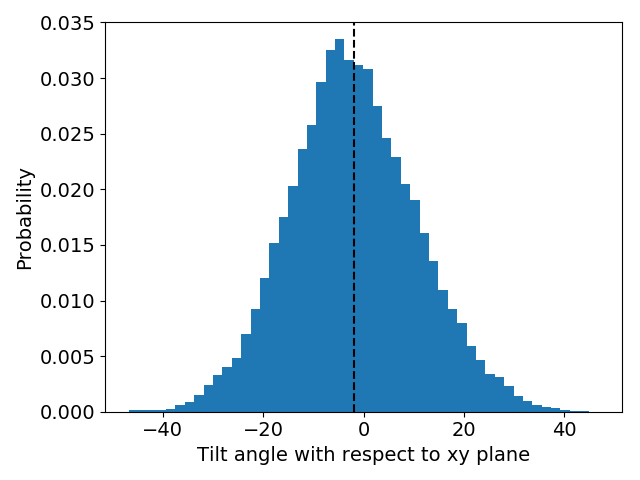
\includegraphics[width=0.5\linewidth]{tilt_dist.png}
  \caption{We measured the angle made between each monomer alkane tail and the
	  membrane plane. The average tilt angle is near 7\degree~which is far from the
	  37\degree~tilt angle previously used to explain R-spots.}~\label{fig:tilt}
  %MRS6: might want to add some discussion about how the angles are also very spread out, so there should be little signal due to tilt anywhere.
  %BJC2: good idea
  \end{figure}

  The peaks in the nearest neighbor angle distribution are consistent with the
  location of R-spots. The peaks of interest in Figures \ref{fig:offset_tails}
  and \ref{fig:layered_tails} are located at $\pm 33 \degree$ which is the same
  location where the highest intensity of spots are located on the simulated
  patterns. We confirmed this conclusion by radially integrating the 2D WAXS
  pattern for $\left|\mathbf{q}\right|$ values between 1.4 and 1.57 (between 4
  and 4.5 \AA~in real space). We observe that distinct peaks appear ca. $30
  \degree$, in close agreement with the previously measured angle distribution
  (Figs.~\ref{fig:offset_integration}~and~\ref{fig:layered_integration}). We
  performed the same integration on the raw experimental data and found the angle
  at which R-spots reaches its highest intensity to be $\pm 37 \degree$ which
  is a reconcilable difference with our simulated results.

  The evidence supports the hypothesis that alkane chain tails pack in a
  hexagonal array. Groups of three tails associated with each monomer prefer to
  sit between tails of vertically stacked monomers rather than stacking directly
  on top of them (Figure~\ref{fig:hex_tails}). This type of packing has been seen
  before in XRD studies of hydrocarbon chains~\cite{small_lateral_1984}.

  \begin{figure}
	\centering
	\begin{subfigure}{0.45\linewidth}
		\centering
	 	\vspace{-2em}
		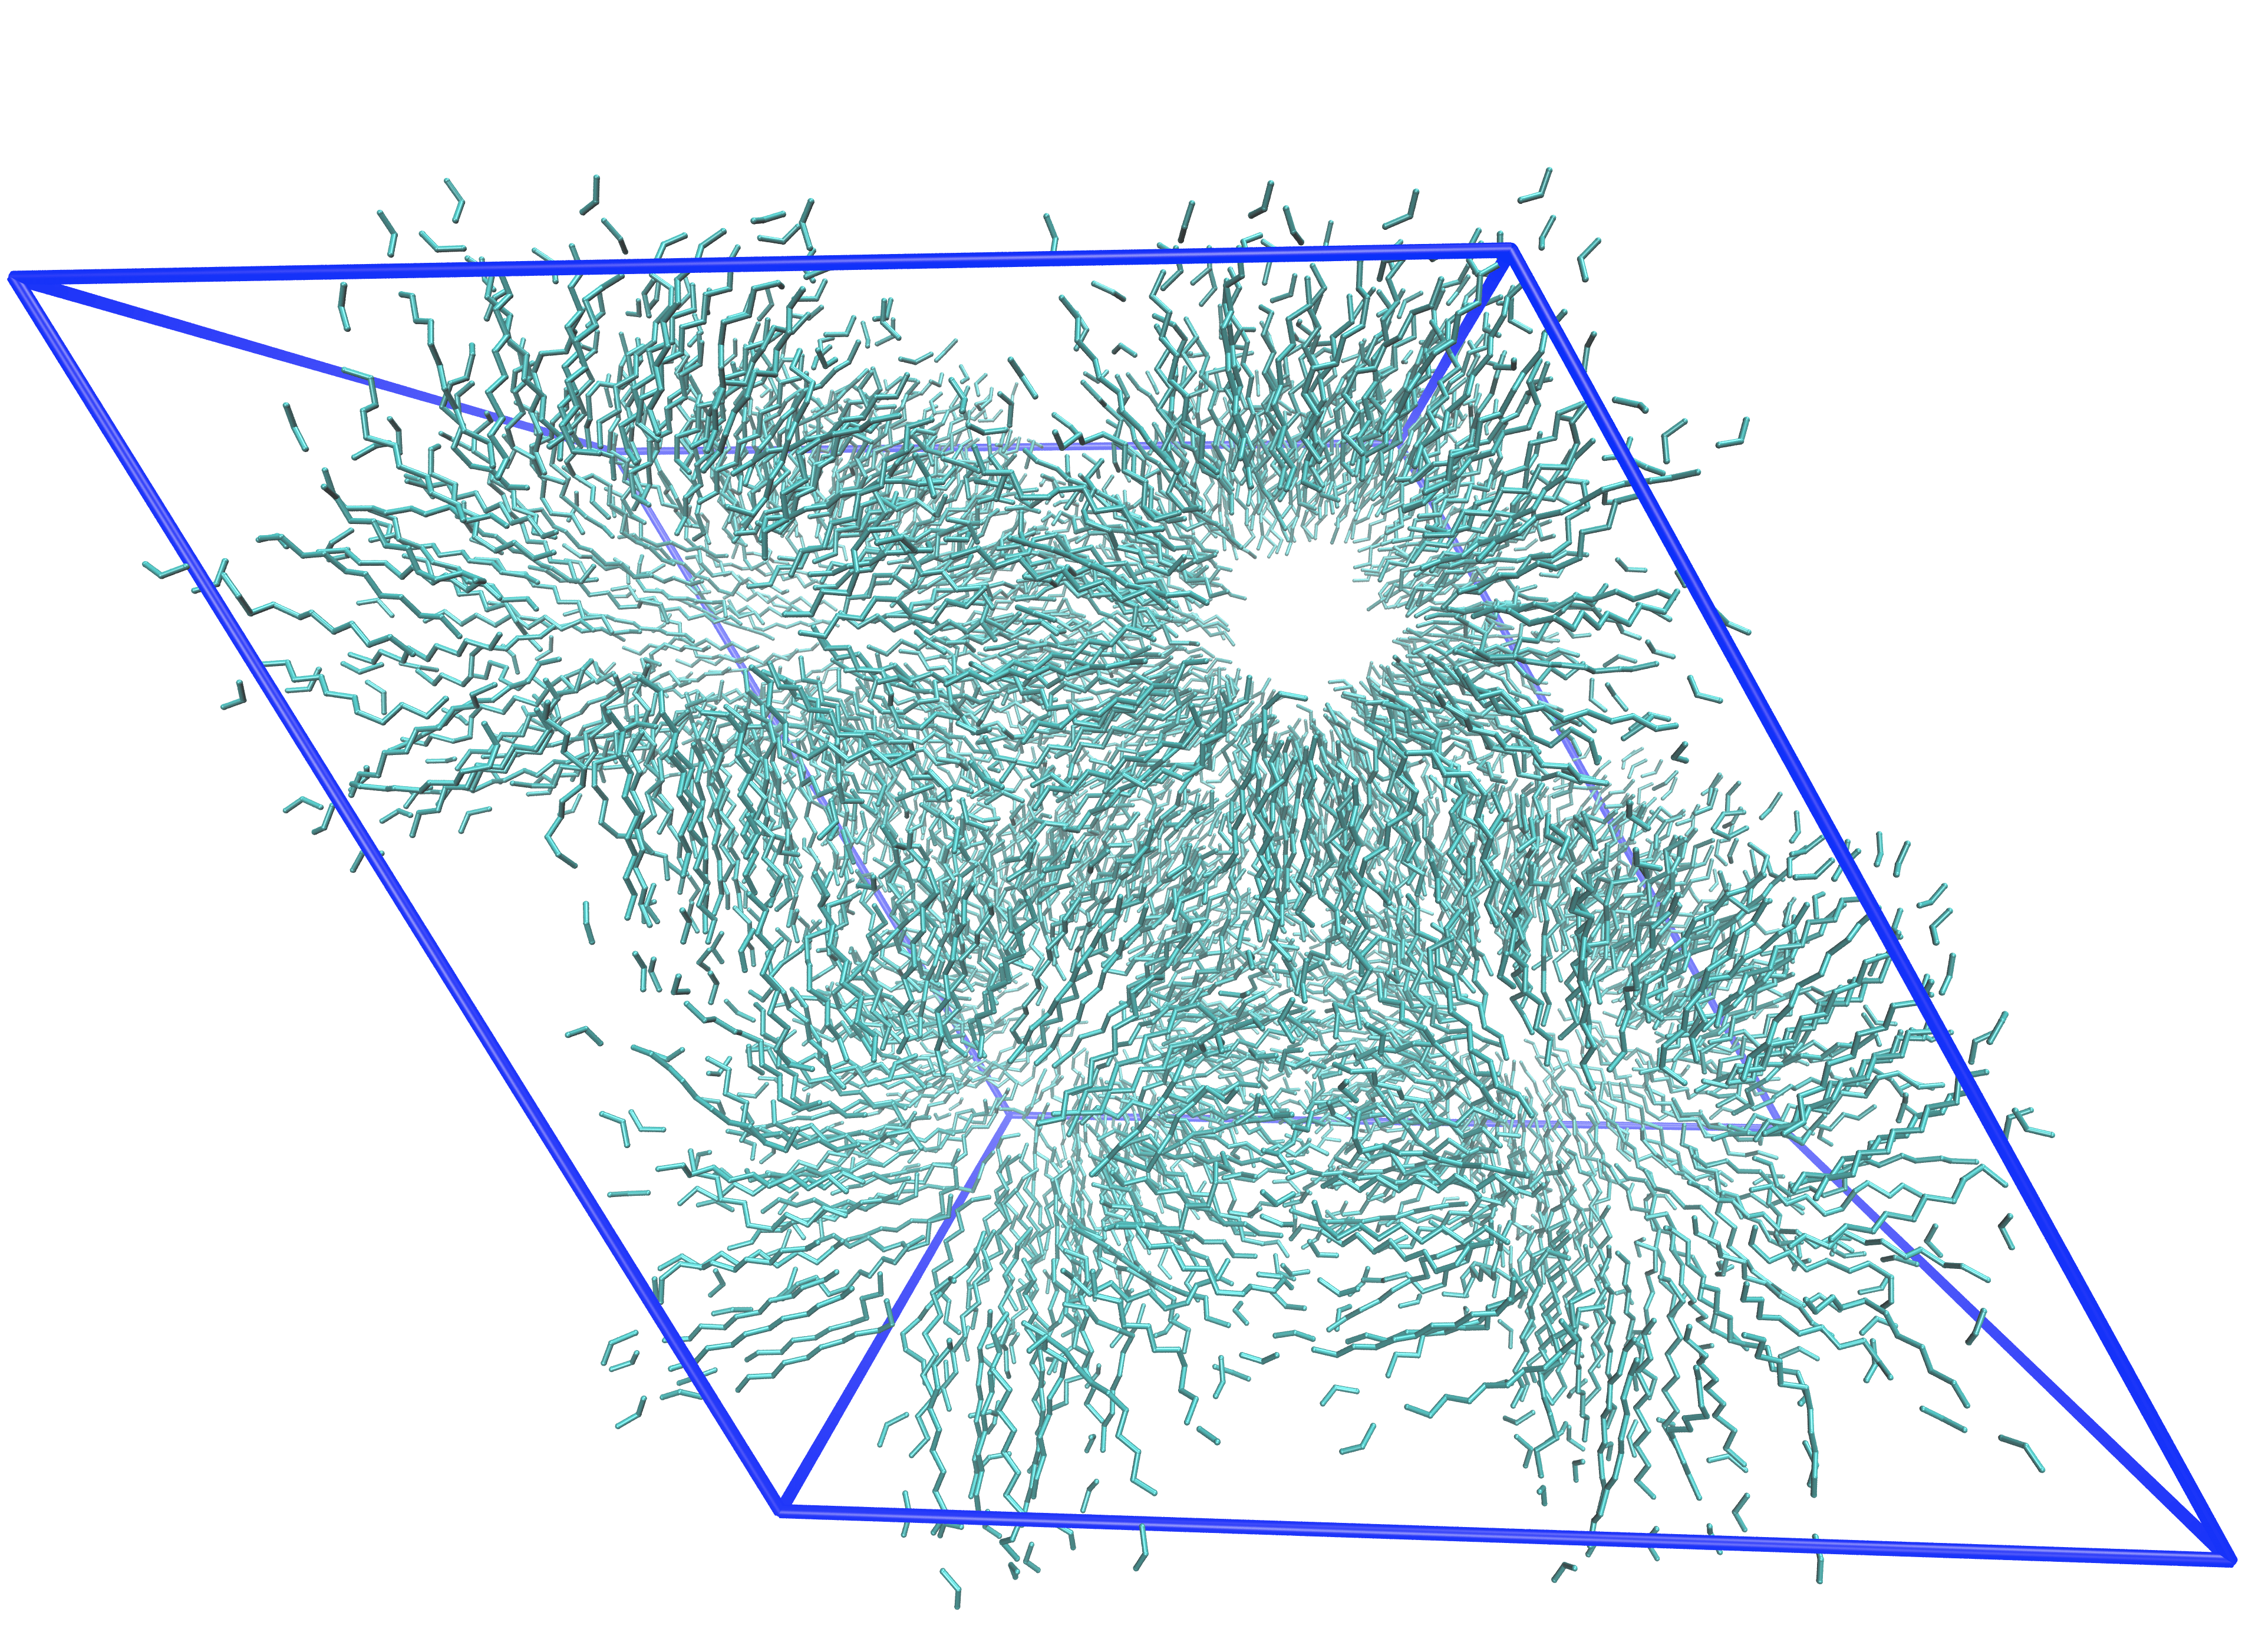
\includegraphics[width=\textwidth]{tails_topview.png}  % picture of top of unit cell with only tail atoms shown
		\caption{}\label{fig:topdown_tails_only}
	\end{subfigure}
	\begin{subfigure}{0.45\linewidth}
		\centering
		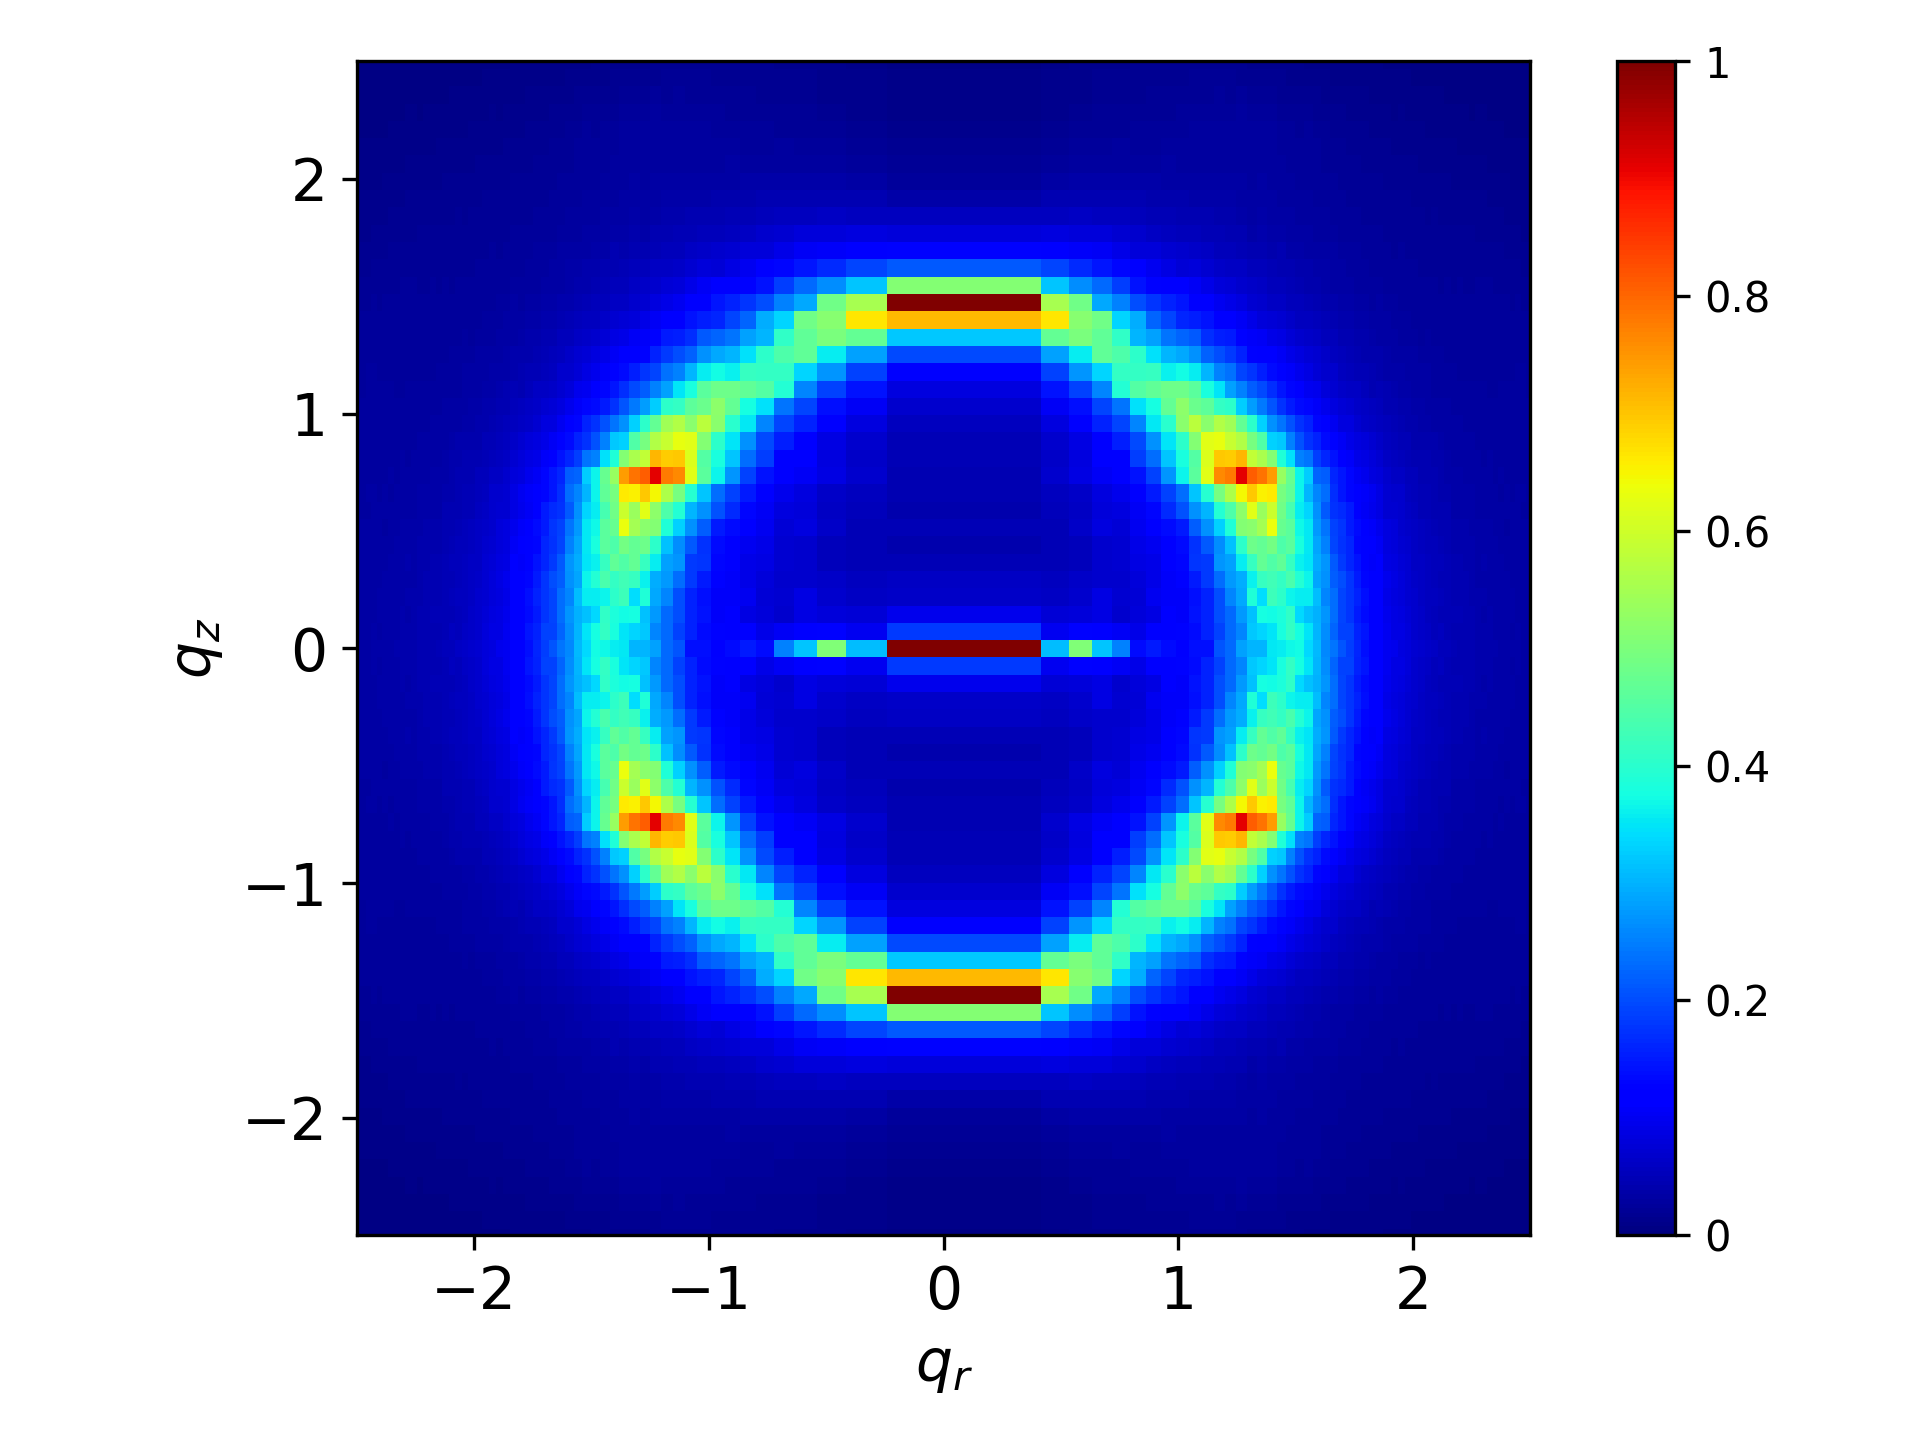
\includegraphics[width=\textwidth]{tails_rzplot.png}
		\caption{}\label{fig:tails_rzplot}
	\end{subfigure}
	\caption{(a) We removed all atoms except carbon atoms that constitute the tails from a 
	sandwiched configuration trajectory. (b) The simulated XRD pattern of the
        tail-only trajectory still shows R-spots}\label{fig:tails}
        %MRS3: so I didn't realize this before, but why are there still fairly significant peaks in the pi-stacking region when the head groups are removed?
        %Do you feel you understand this? I suppose it is because the top of the tails must be correlated with the aromatic ring by covalent bonding?
        %BJC2: Yea, I think the reflection is correlated to the aromatic rings. The system shown is the sandwiched configuration. The intensity of "R-pi"
        % in this pattern is lower than in the pattern generated by the full system. The aromatic rings appear to strengthen the reflection. 
        % Also, the system is layered in the z-direction, as we show, so a reflection like that should appear. 
        %MRS4: did you use a different scaling for the color bar here than above? If so, mention.
        %BJC3: The scaling is the same
        %MRS6: OK, I'm seeing this new light. the HUGE intensity in the simulation is from the carbon of the tail, not the pi-pi. There isn't anything like that in the experimental in the alkane region.  What happens if you remove a couple of more carbons from the tails? Does this has something to do with the stacking of alkane tails in the z direction? is that not experimentally observed? I need to think through this a bit more . . .  I maybe missing something obvious having to do with require correlations between the stacking of the tails and the stacking of the pi.  Maybe normalizing by the tails is NOT the right thing to do, because in the z direction, stacked pi interactions lead to stacked tails at the same distance (a requirement of the molecules being connected, so if that stacking is different between experiment and theory, it leads to different intensities.  On the other hand, if the experiment had tails that are stacked together at 3.7 A on average, it seems like they would have to be much flatter to fit.  Hmmm.  What do the aromatics signals alone look like? (i.e. the opposite of 9a). I need to think . . . 
  \end{figure}

  \begin{figure}[!htb]
  \centering
  	\begin{subfigure}{\linewidth}
	\centering
		\begin{subfigure}{0.45\textwidth}
        		\centering
        		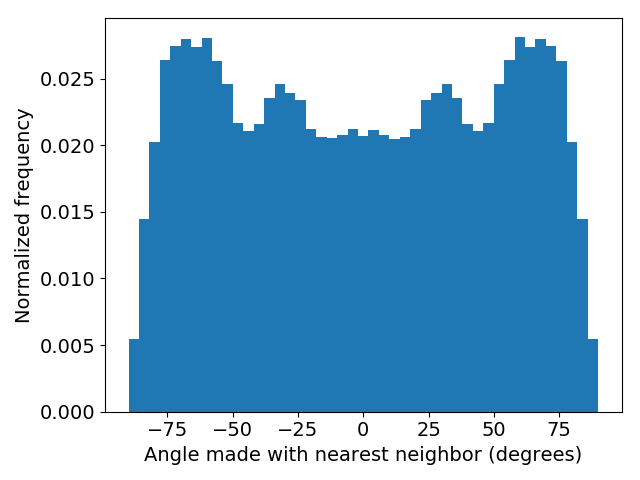
\includegraphics[width=\linewidth]{offset_tail_packing.png}
        		\caption{}~\label{fig:offset_tails}
		\end{subfigure}
		\begin{subfigure}{0.45\textwidth}
		\centering
	        	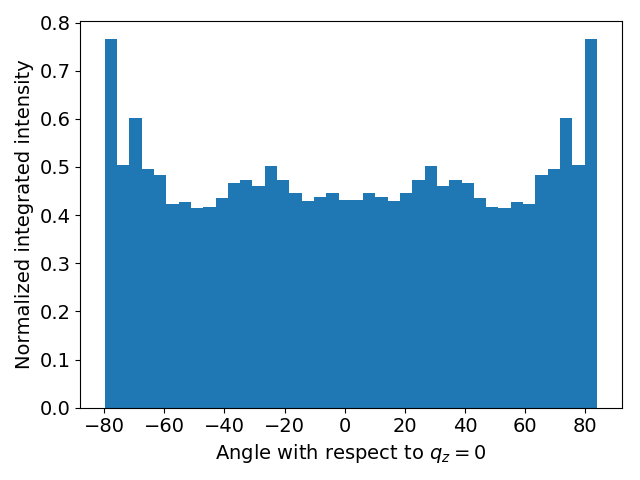
\includegraphics[width=\linewidth]{offset_angle_v_I.png}
		        \caption{}~\label{fig:offset_integration}
		\end{subfigure}
	\end{subfigure}
	\begin{subfigure}{\linewidth}
	\centering
		\begin{subfigure}{0.45\textwidth}
	        \centering
		        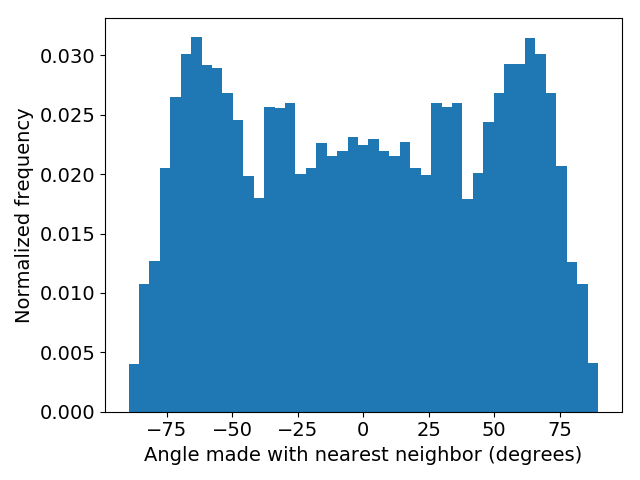
\includegraphics[width=\linewidth]{angles_traj_layered.png}
		        \caption{}~\label{fig:layered_tails}
		\end{subfigure}
		\begin{subfigure}{0.45\textwidth}
        	\centering
		        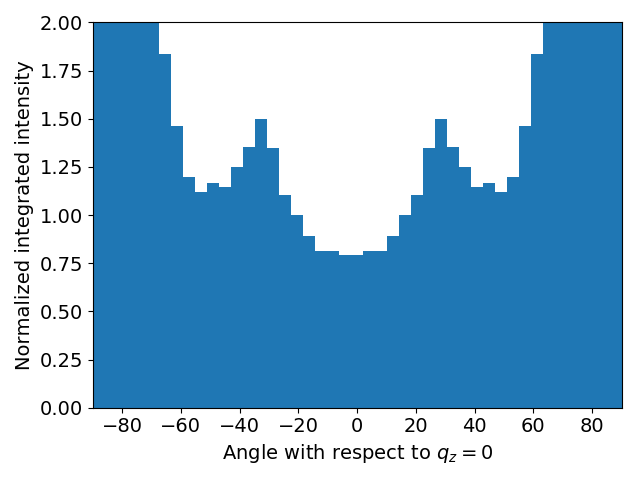
\includegraphics[width=\linewidth]{layered_angle_v_I.png}
		        \caption{}~\label{fig:layered_integration}
		\end{subfigure}
	\end{subfigure} 
  \caption{We hypothesize that R-spots is the result of ordered tail packing.
	  Defining the membrane plane to be 0\degree, we measured the angles between each
	  alkane chain tail centroid and its nearest neighbor centroids for the
	  equilibrated parallel displaced (a) and sandwiched (c) configurations. Peaks
	  that appear in each distribution are centered near $\pm~33\degree$. We radially
	  integrated the simulated XRD patterns of the parallel displaced and sandwiched
	  configuration within the region bounding R-alkanes ((b) and (d) respectively).
	  Peaks appear in the same location as the angle distributions which corroborates
	  our hypothesis. Further, we note that the peaks are strongest in both plots
	  associated with the sandwiched configuration. As shown in Figure
	  \ref{fig:rz_layered}, systems simulated in the sandwiched configuration exhibit
	  more intense R-spots reflections. Note that plots of integrated intensity are
	  normalized so the average alkane intensity (excluding reflections $\pm
	  30\degree$ from the $q_z$ axis) is set to 1.  Plots are cut off for intensities
	  greater than 2 so peaks are more visible.}~\label{fig:tail_packing}
  \end{figure}

%BJC: not sure if this figure is necessary.  
%MRS6: kind of confusing with just the circles and no molecules to hang them on.
  \begin{figure}
	\centering
	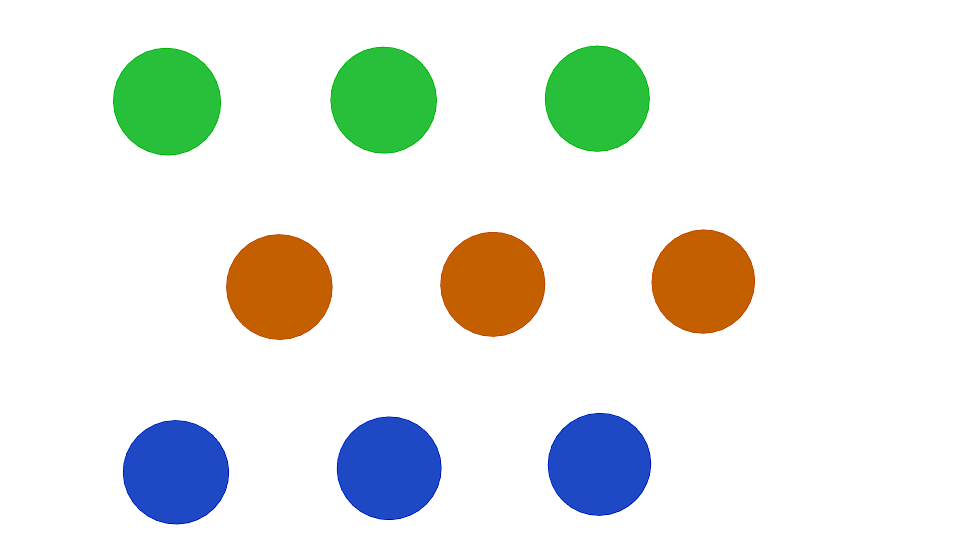
\includegraphics[width=0.5\linewidth]{hexagonal_tails_alt2.png} 
	%BJC: I can give the circle some depth if that makes it clearer
	\caption{Monomer tails prefer to pack in a hexagonal array. Each circle
		represents a monomer tail as seen if viewed by looking from the end of the tail
		to the pore center. Each color represents distinct monomers from adjacent
		layers.}~\label{fig:hex_tails}
  \end{figure}
	
  \subsubsection{Layer partitioning}

%MRS6: should probably be present tense.  Maybe phrase ``in our simulations, layers are'' 
  In our simulations, layers are well-defined and persistent, answering question
  (\ref{point:layers}). We established our conclusion by plotting the two
  dimensional pair distribution function, $g(y,z)$ of head group phenyl rings
  using Equation~\ref{eqn:correlation} (Figure \ref{fig:yz_correlation}). In both
  configurations, the phenyl rings stack in the z-direction, along $y=0$, and
  clear layers are formed. The layers in the sandwiched configuration are more
  defined than those in the parallel displaced configuration and are strongly
  correlated with adjacent layers. We also observe correlation of layers between
  pores indicated by the non uniformity in $g(y,z)$ in adjacent columns (along $y
  = \pm 3.65$). Parallel displaced layers display weaker correlations but do not
  decay in their intensity as z increases. We do not see correlation between
%MRS6: correlations of what between pores?
  pores, however correlations within pores are strong throughout the length of
  the unit cell since there is no noticeable decay in layer intensity. 

  \begin{figure}
  \centering
  \begin{subfigure}{0.45\textwidth}
	\centering
	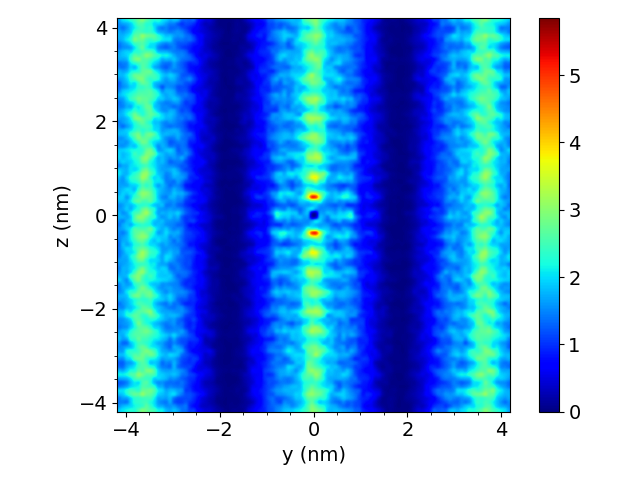
\includegraphics[width=\textwidth]{layered_yz_correlation.png}
	\caption{}\label{fig:layered_yz_correlation}
  \end{subfigure}
  \begin{subfigure}{0.45\textwidth}
        \centering
        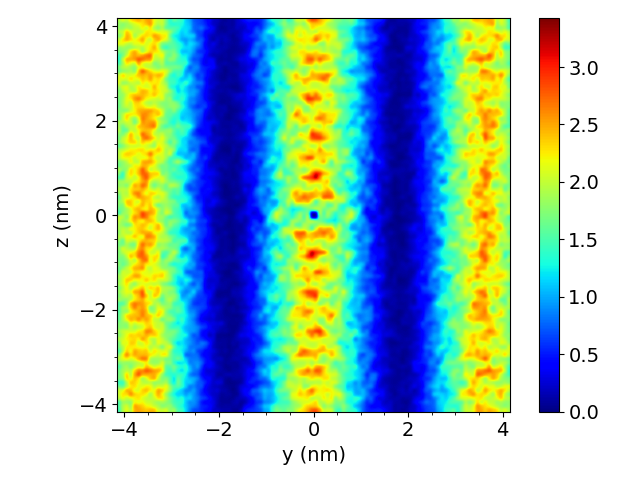
\includegraphics[width=\textwidth]{offset_yz_correlation.png}
        \caption{}\label{fig:offset_yz_correlation}
  \end{subfigure}
  %MRS6: have the same color scale in both figures to compare them?
  \caption{2D pair distribution functions generated from systems built in the 
	   sandwiched (a) and parallel displaced (b) configurations, provide
           a more detailed picture of the pore structure in each. The sandwiched
	   configuration}\label{fig:yz_correlation}
%MRS6: caption not finished?
  \end{figure} 

  We plotted the one-dimensional pair distribution function, $g(z)$, for the
  phenyl rings and for carbon atoms that make up the monomer tails (Figure
  \ref{fig:zdf}). The plots show clear periodic maxima where layers are present.
  Layering is most pronounced in the head group region, however there is still a
  degree of layering that persists into the tail region. Using a Fourier
  transform on $g(z)$ from the head groups, we see that sandwiched configuration
  layers stack 4.39 \AA~apart while parallel displaced configuration layers stack
  4.38 \AA~apart. Both stacking distances are in agreement with those observed
  in the simulated XRD patterns.

  %MRS6: do you need both the 2D and 1D correlation functions?
  \begin{figure}
        \centering
        \begin{subfigure}{0.45\textwidth}
                \centering
                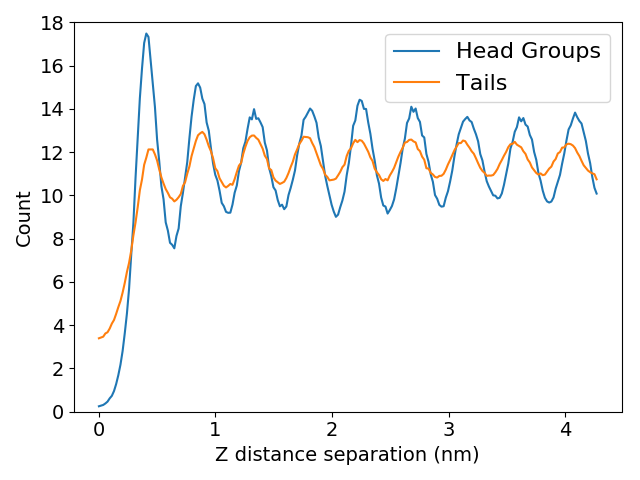
\includegraphics[width=\textwidth]{zdf_overlay_layered.png}
                \caption{}\label{fig:zdf_layered}
        \end{subfigure}
        \begin{subfigure}{0.45\textwidth}
                \centering
                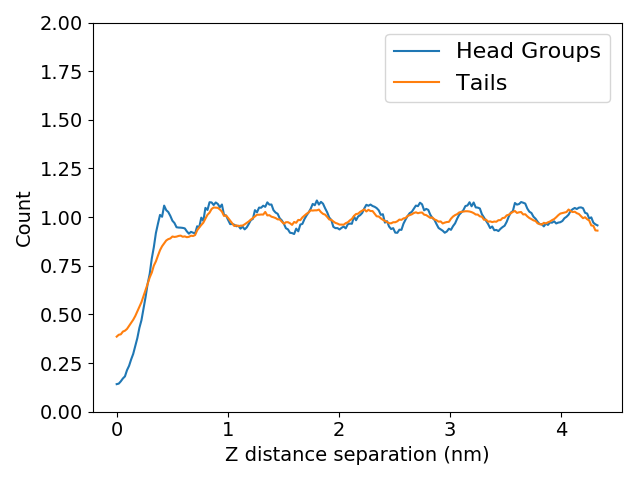
\includegraphics[width=\textwidth]{zdf_overlay_offset.png}
                \caption{}\label{fig:zdf_offset}
        \end{subfigure}
	\caption{We support the existence of layers with the observance of
		clear periodic maxima in the $z$-direction pair distribution functions of the
		(a) 5 monomer per layer, sandwiched and (b) 5 monomer per layer, parallel
		displaced configurations. The extent to which we consider a system to be
		layered is based on the magnitude of the deviation of the periodic maxima from
		the average number density. The sandwiched configuration possesses a higher
		degree of layering than the parallel displaced configuration and, in both
		cases, the head group region has a higher degree of layer partitioning than the
		tail region. (See Supporting information for detailed definitions of the head
		group and tail regions)}\label{fig:zdf}
  \end{figure}

  \subsubsection{Initial Layer Spacing Affects System Equilibration}

  All systems up to this point were built with layers stacked 3.7 \AA~apart.
  When we build systems with layers stacked 5.0 \AA~apart and then let them
  equilibrate, we observe long-term stability of a qualitatively different
  configuration, suggesting that we have found another metastable free energy
  basin, further corroborating question (\ref{point:metastable}). 
  %The basins are
  %differentiated by their relative degrees of ordering resulting from different
  %spatial arrangements. 
  For reasons we will develop in the next segment of our
  discussion, configurations intially built with layers stacked 5.0 \AA~apart 
  will be grouped into the disordered pore basin, while those built with layers
  initially stacked 3.7 \AA~apart will be grouped into the ordered pore basin.

  The equilibrated pore spacing and distance between layers are different in
  the disordered pore basin. For both head group stacking arrangements, we
  observe an increase in the equilibrated distance between layers
  (Fig.~\ref{fig:dbwl_disordered}) and a corresponding decrease in pore spacing
  (Fig.~\ref{fig:p2p_disordered}).

  The simulated X-ray diffraction patterns indicate further structural
  differences. In the parallel displaced configuration, almost all contrast
  between R-spots and R-alkanes fades (Figure~\ref{fig:offset_disordered_xrd}).
  In the sandwiched configuration, R-spots is present, but there are only two
  spots located at the intersection of $q_z=0$ with R-alkanes.
  (Figure~\ref{fig:layered_disordered_xrd}). 

% BJC: in the interest of being concise, I leave this out for now.
%  The sandwiched and parallel displaced assemblies do not deviate from their
%  initial head group arrangement. R-helix is still faintly visible in the
%  parallel displaced configuration and is absent in the sandwiched simulated
%  diffraction pattern. The spectroscopic signatures are unique to the two
%  different head group configurations.

  \begin{figure}[!hbt]
        \centering
        \begin{subfigure}{0.45\linewidth}
                \centering
                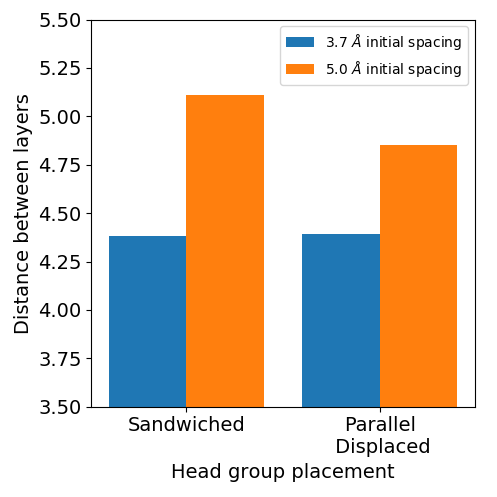
\includegraphics[width=\linewidth]{dbwl.png}
                \caption{}~\label{fig:dbwl_disordered}
        \end{subfigure}%
        \begin{subfigure}{0.45\linewidth}
                \centering
                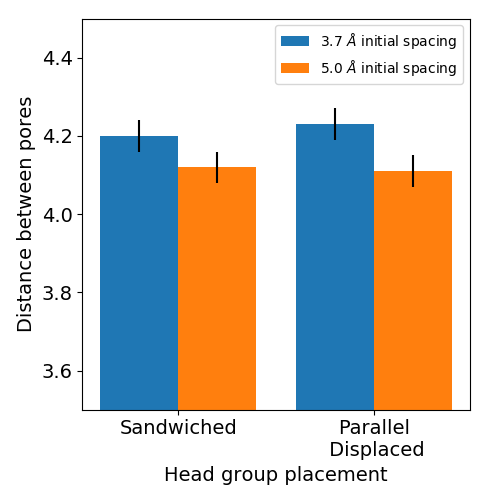
\includegraphics[width=\linewidth]{p2p2.png}
                \caption{}~\label{fig:p2p_disordered}
        \end{subfigure}
        \begin{subfigure}{0.45\linewidth}
                \centering
                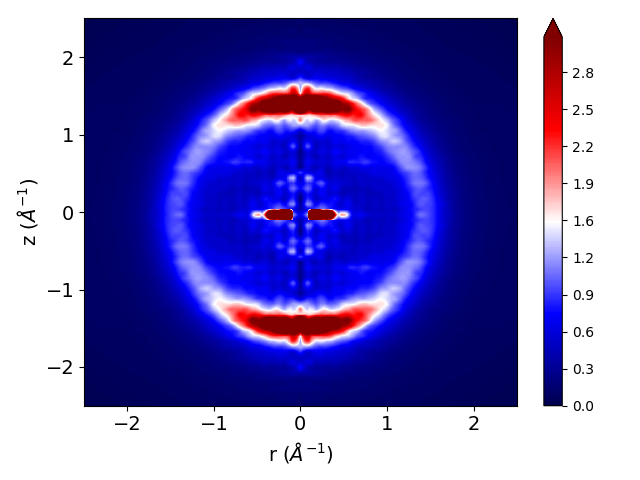
\includegraphics[width=\linewidth]{disorder_offset_rzplot.png}
                \caption{}~\label{fig:offset_disordered_xrd}
        \end{subfigure}%
        \begin{subfigure}{0.45\linewidth}
                \centering
                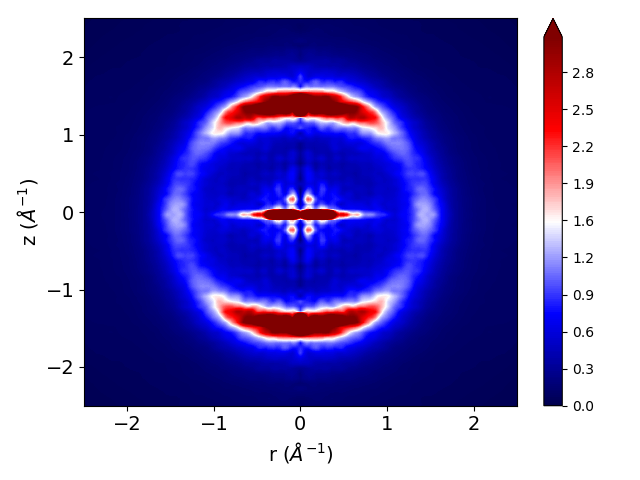
\includegraphics[width=\linewidth]{disorder_rzplot.png}
                \caption{}~\label{fig:layered_disordered_xrd}
        \end{subfigure}
	\caption{There are distinct differences between the disordered and ordered pore systems. 
		When layers are initially stacked 5\AA~ apart, the distance
		between layers increases (a) and the pore spacing decreases (b) in comparison to
		the ordered pore systems. The simulated
		XRD patterns of disordered pore systems are also appreciably different, most 
		notably in the region bounded by R-alkanes. The disordered pore
		systems started in the parallel displaced configuariton (c) does not show R-spots
		or R-$\pi$ which suggests that head groups are not associating with each other
		and tails are distributed nearly isotropically. The disordered pore system
		started in the sandwiched configuration (d) does not show R-$\pi$ but R-spots 
		is present in different locations because the tails are packed in a different
		motif.}
  \end{figure}

  %BJC: this may belong in methods, but I think it might fit here because it
  % gives context for the choice of functional form to fit

  We quantified order in the z-direction by measuring the correlation lengths
  of all configurations. We measured the correlation length, L, by fitting $g(z)$
  using a non-linear least squares algorithm subject to a function of the form:
  \begin{equation}
  	1 + Asin(Bx + C)e^{-z/L}
        \label{eqn:correlation_fit}
  \end{equation}
  where z is the independent variable and all other variables are fitting
  parameters. The correlation length for each system is given in
  Table~\ref{table:nematic}.

  Correlation lengths are shorter in the disordered pore basin than in the
  ordered pore basin. Layers in the ordered pore basin are strongly correlated
  with neighboring layers up to more than 10 layers away. This behavior deviates
  from experimental evidence. The experimental correlation length (See
  Suppporting Information for details its derivation) suggests that layers are
  correlated with about 3 neighboring layers which is closer to the values
  exhibited by the disordered pore basin. We may need to simulate a system with
  many more layers in order to reduce the correlation contributed by periodic
  copies of the system. 

%MRS6: not sure if we WANT to do this, but could do a simulation with 2x as many layers and see if the correlation changes.
%BJC2: have one that is 3x going right now

  We calculated the nematic order parameter for each system using Equation
  \ref{eqn:nematic_order_parameter}. The calculated values of S are presented in
  Table \ref{table:nematic}. The full distributions of angles between director
  \textbf{n} and vectors orthogonal to monomer phenyl rings are presented in the
  Supporting Information. In general, ordered pore basin systems are more
  nematically ordered than disordered pore basin systems and sandwiched
  configuration systems are more nematically ordered than parallel displaced
  configuration systems. The head groups of the disordered pore basin have more
  rotational freedom about the xy plane likely due to the larger separation
  between layers. Similarly, monomers situated in the sandwiched configuration
  are constrained by other monomers stacked directly above and below them, while
  monomers in the parallel displaced configuration have no direct neighbors
  vertically which provides them with more rotational freedom. 

  \begin{table}[h]
  \centering
  \begin{tabular}{ccc}
  \toprule
  System & Correlation Length (\AA) & Nematic Order Parameter (S) \\
  \midrule
  Sandwiched, Ordered & 41 $\pm$ 3 & 0.659 $\pm$ 0.003 \\
  Parallel Displaced, Ordered & 86 $\pm$ 14 & 0.601 $\pm$ 0.003 \\
  Sandwiched, Disordered & 17 $\pm$ 3 & 0.565 $\pm$ 0.002 \\
  Parallel Displaced, Disordered & 9 $\pm$ 1 & 0.503 $\pm$ 0.002 \\
  Experiment & 10 $\pm$ 1 & -- \\
  \bottomrule
  \end{tabular}
  \caption{The nematic order parameter, S, is higher when layers are initially spaced
  3.7 \AA apart. In general, the sandwiched configuration has higher nematic order
  than the parallel displaced configuration. Correlation lengths are higher in
  the ordered pore basin. Correlation lengths in the disordered pore basin are
  in closer agreement with experiment. WHY IS THIS BOLD??!}~\label{table:nematic}
%MRS6: for some reason, might be set in the jpcbfk package?
  \end{table}

%  \begin{table}[h]
%  \centering
%  \begin{tabular}{ccc}
%  \toprule
%  System & Layer Separation & Correlation Length \\
%  \midrule
%  Sandwiched & 4.39 \AA & 41 $\pm$ 3 \AA \\
%  Parallel Displaced & 4.38 \AA & 86 $\pm$ 14 \AA \\
%  Experiment* & 3.7 \AA & 10 $\pm$ 1 \AA \\  
%  \bottomrule
%  \end{tabular}
%  \caption{Uncertainties are derived from the diagonal entries in the
%	  covariance matrix calculated from a non-linear least squares fit to the data.
%	  *See supplemental information for derivation of experimental correlation
%	  length}~\label{table:correlation_length}
%  \end{table}

  %BJC: this might be better situated before the numerical calculations that go 
  %into Table 1
  We observe evidence of disorder in the xy plane of the disordered pore basin when
  we plot the two dimensional pair distribution function, $g(x,y)$, between the
  centers of mass of monomer phenyl rings (Figure \ref{fig:xy_correlation}). The
  difference is most apparent in the plots of the sandwiched configurations. In
  the ordered pore basin, head groups primarily stay stacked on top of each other
  while in the disordered pore basin, head groups exhibit more motion about the pore
  center and even drift into the middle of the pore. $g(x,y)$ for the parallel displaced
  configuration is less informative since adjacent layers are displaced in a way that
  occupies the gaps that are seen in $g(x,y)$ for the sandwiched configuration 

  \begin{figure}
  \begin{subfigure}{1\linewidth}
        \centering
        \begin{subfigure}{0.47\linewidth}
                \centering
                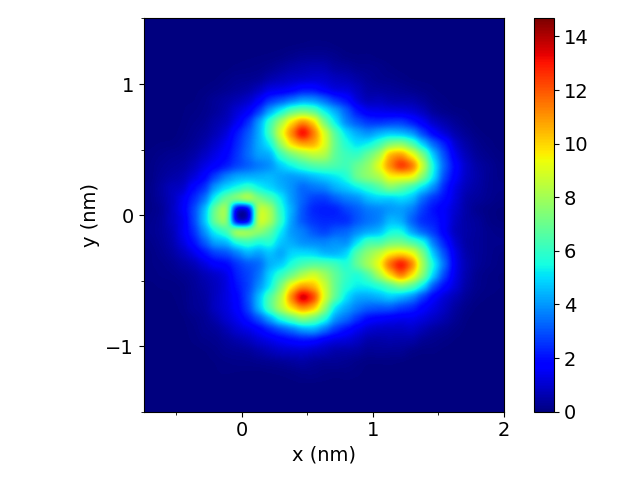
\includegraphics[width=\linewidth]{layered_xy_correlation.png}
                \caption{Sandwiched, Ordered Pore Basin}~\label{fig:sandwich_xy}
        \end{subfigure}
        \begin{subfigure}{0.47\linewidth}
                \centering
                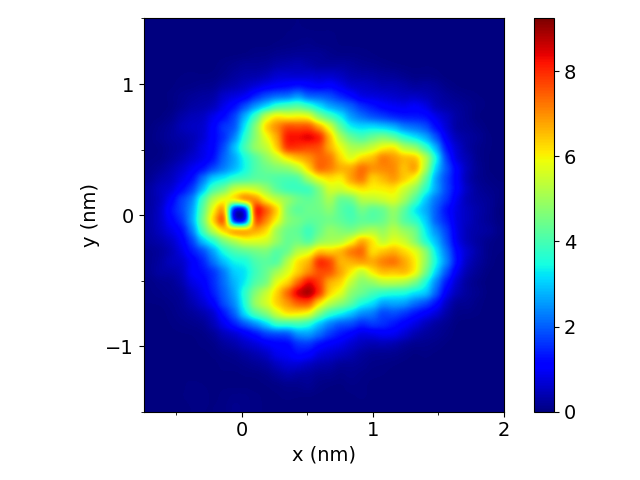
\includegraphics[width=\linewidth]{disorder_xy_correlation.png}
                \caption{Sandwiched, Disordered Pore Basin}~\label{fig:disorder_sandwich_xy_correlation}
       \end{subfigure}
       \begin{subfigure}{0.47\linewidth}
                \centering
                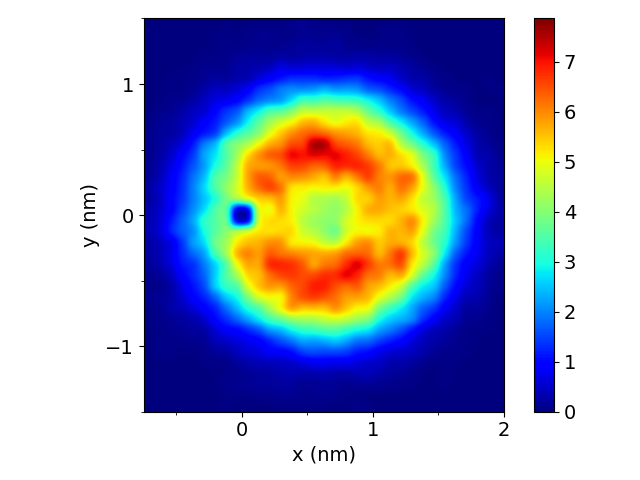
\includegraphics[width=\linewidth]{offset_xy_correlation.png}
                \caption{Parallel Displaced, Ordered Pore Basin}~\label{fig:offset_xy}
        \end{subfigure}
        \begin{subfigure}{0.47\linewidth}
                \centering
                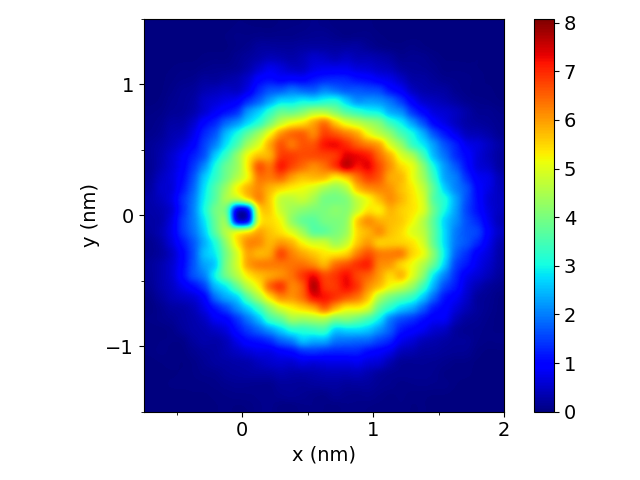
\includegraphics[width=\linewidth]{disorder_offset_xy_correlation.png}
                \caption{Parallel Displaced, Disordered Pore Basin}~\label{fig:disorder_offset_xy_correlation}
        \end{subfigure}
  \end{subfigure}
  \caption{$g(x,y)$ for sandwiched and parallel displaced configurations in the
	  ordered and disordered pore basins illustrates the increase in xy plane
	  disorder when initial configuration layer stacking distance is increase from
	  3.7 \AA~to 5 \AA~apart.}\label{fig:xy_correlation}
  \end{figure}

  \subsection{Slow dynamics}
%MRS6: Is the fact that it's lyotropic relevant? 
  We observe unusually slow dynamics in our system. Typical diffusion constants
  for columnar liquid crystals have been reported to be on the order of
  $10^{-11}~ m^2/s$ \cite{dong_translational_1984}. We measured the diffusion
  constants of monomers in each of the systems we studied (Table~\ref{table:msd})
  and learned that they are all on the order of $10^{-14}~m^2/s$. Our systems may
  be frozen in a glassy state. It is also possible that we are simply observing
  characteristics of the experimental system. There has been no experimental work
  done to study diffusion of NA-GA3C11 monomers in the Col\textsubscript{h}
  system and no measurement of the glass transition temperature. Such a low
  diffusion constant is not unheard of. A more recent study reported a diffusion
  constant of $1.2\times10^{-14}~m^2/s$ for a different liquid crystal that
  formed a hexagonal columnar phase \cite{dvinskikh_molecular_2002}. 

%MRS6: I don't know that the equilibration procedure induces it; I doubt a metastable state would have slower kinetics than the real state. It might be the force field is too stable. 
  It is possible that our equilibration procedure may induce glassy phase
  configurations. We have already shown that our system has some dependence on
  initial configuration. It is conceivable that after a fast initial relaxation,
  the system gets locked into a structure close to its initial configuration.
  The glassy state of these systems may be the reason we observe such high
  correlation lengths in the ordered pore basin systems.  Unfortunately, we are
  unable to resolve the exact atomistic structure using existing experimental
  techniques, so we are left to find out which initial configuration results in a
  model with the closest match to experimental data.
%MRS6: don't need a table if all the same.
  \begin{table}[h]
  \centering
  \begin{tabular}{cc}
  \toprule
  System & Diffusion Constant ($m^2/s$) \\ 
  \midrule
  Sandwiched, Ordered & $10^{-14}$ \\
  Parallel Displaced, Ordered & $10^{-14}$ \\
  Sandwiched, Disordered & $10^{-14}$ \\
  Parallel Displaced, Disordered & $10^{-14}$ \\
  \bottomrule
  \end{tabular}
  \caption{The diffusion constants for all systems are on the order of $10^{-14} m^2/s$ 
  which is three orders of magnitude lower than literature values.}~\label{table:msd}
  \end{table}

  \subsubsection{Chemical composition of pore columns}

%MRS: I think you will need to refer back to names of the questions (or at least shortened versions of the names): people skimming the paper will not remember what the numbers are.
  In order to address question (\ref{point:poredefinition}), we plotted the
  number densities of heavy atoms in the head group, carbon atoms in the tail
  region and all sodium ions (Figure~\ref{fig:densities}). For the head group
  region, we used the carbon atoms making up the aromatic ring. For the tail
  region we used only carbon atoms of the monomer tails (See Supporting
  Information for diagram). We average the histograms over at least 50 ns of
  equilibrated trajectory.
  
  In all cases, the space in the pore region is filled with sodium ions and
  head groups. Systems in the ordered pore basin are less dense in
  the center of the pore. In both the sandwiched and parallel displaced
  configurations, we see the density of head groups and sodium ions fall to less
  than 50\% of its maximum at r = 0 (Fig.~\ref{fig:layered_density}). The
  situation is most pronounced in the sandwiched configuration where the maximum
  head group density occurs 0.44 nm from the pore center. The parallel displaced
  configuration reaches its maximum 0.35 nm from the pore center. In contrast,
  both disordered pore systems show very little difference in density from its
  maximum. This implies a more uniform distribution of head groups within the
  pore center. This is the same conclusion drawn from the plots of $g(x,y)$ 
  (Figure~\ref{fig:xy_correlation}). 
  % High vacancy is less likely to be stable in the real system

  There is a partition between the hydrophobic and hydrophilic regions, however
  it is a gradient in composition, rather than an abrupt division. The system
  does not confine sodium ions and head groups to just within the pore region.
  Assuming a pore radius of 0.6 nm, we see in all cases, that 19\% of sodium ions
  exist outside the pore region (except sandwiched, ordered pore, where 16\%
  are outside the pore). Additionally, we see that in all cases, about 3\% of the
  plotted tail density is located within the pore region (except sandwiched,
  ordered pore, where 1.5\% are within the pore region). These observations bring
  into question how one should define a pore in these types of systems. One
  usually measures a membrane's pore radius based on the size of a molecule it
  can reject, however it is not clear where the edges of the pores are and what
  size molecule would fit through. We leave these investigations for a future
  study.

  \begin{figure}
  \centering
  \begin{subfigure}{0.47\textwidth}
        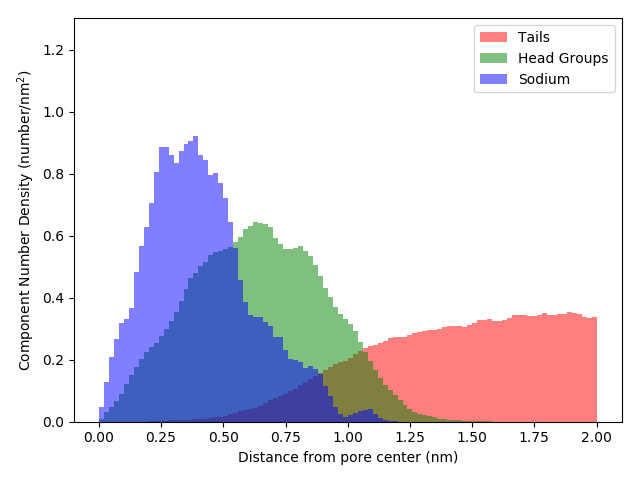
\includegraphics[width=1\linewidth]{offset_density.png}
        \caption{Parallel Displaced, Ordered Pore Basin}
        \label{fig:offset_density}
  \end{subfigure}
  \begin{subfigure}{0.47\textwidth}
        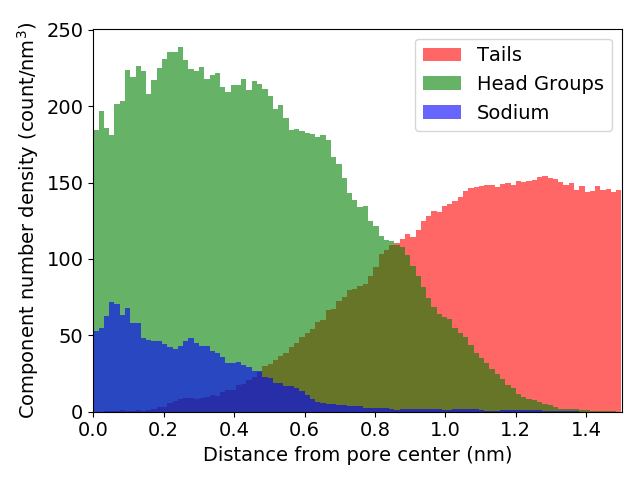
\includegraphics[width=1\linewidth]{layered_density.png}
        \caption{Sandwiched, Ordered Pore Basin}
        \label{fig:layered_density}
  \end{subfigure}
  \begin{subfigure}{0.47\textwidth}
        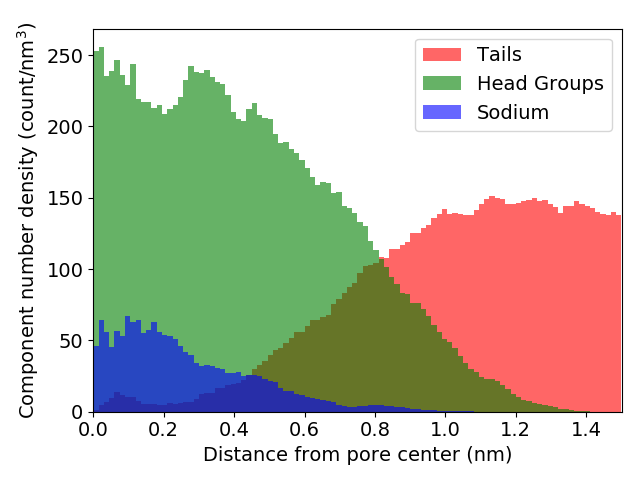
\includegraphics[width=1\linewidth]{disordered_offset_density.png}
        \caption{Parallel Displaced, Disorderd Pore Basin}
        \label{fig:disordered_offset_density}
  \end{subfigure}
  \begin{subfigure}{0.47\textwidth}
        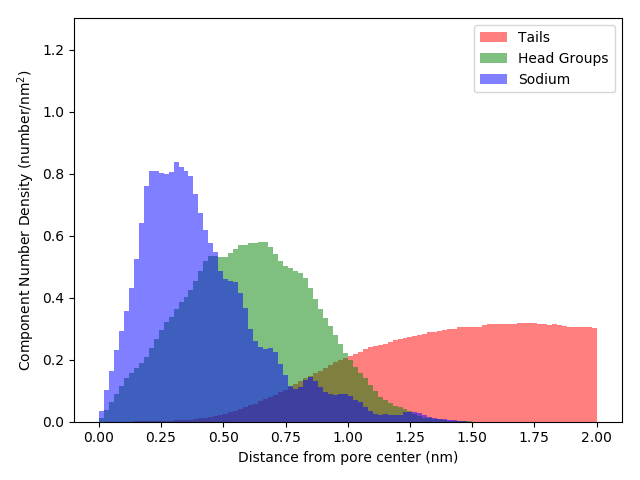
\includegraphics[width=1\linewidth]{disordered_density.png}
        \caption{Sandwiched, Disordered Pore Basin}
        \label{fig:disorder_layered_density}
  \end{subfigure}
  \caption{In all cases, the component radial distribution functions exhibit a
	  composition gradient transitioning from the hydrophilic to the hydrophobic
	  regions. Systems with layers initially spaced 3.7 \AA~apart in the  parallel
	  displaced (a), and sandwiched (b) configurations both show the highest
	  concentrations of ions and head groups away from the pore center. Systems with
	  layers initially spaced 5 \AA~apart (c) and (d), both show the highest
	  concentrations of ions and head groups near the pore center, implying a more
	  uniform, disordered pore.}~\label{fig:densities}
  \end{figure}

  \subsection{Effect of Water on Structure}

  % BJC: I'm not sure this section is necessary anymore. The original point was to 
  % see if we get more structure. It's not clear this is the right way to introduce
  % water into the system. I think it confuses things. 

  %MRS6: good question.  It is interesting to see the swelling. We can talk.

  We explored the affect of water on pore structure, addressing question
  (\ref{point:water}), by preparing parallel displaced and sandwiched
  configurations according to the wet equilibration procedure. There is no
  experimental measurement of trace water concentration in the pores so we tested
  a range of water concentrations from 1 to 5 percent. Our lower bound models a
  system with on average 2 water molecules for each monomer layer.
  % BJC: double check this^ calculation or omit
  Figure~\ref{fig:solvation} shows the simulated diffraction patterns resulting
  from each configuration.

  % formatting taken from : https://tex.stackexchange.com/questions/239715/add-titles-for-rows-and-columns-in-a-subfloat
  \newlength{\tempdima}
  \newcommand{\rowname}[1]% #1 = text
  {\rotatebox{90}{\makebox[\tempdima][c]{\textbf{#1}}}}
  
  \renewcommand{\thesubfigure}{\alph{subfigure}}
  \newcommand{\mycaption}[1]% #1 = caption
  {\refstepcounter{subfigure}\textbf{(\thesubfigure) }{\ignorespaces #1}}
  
  \begin{figure}
  	\settoheight{\tempdima}{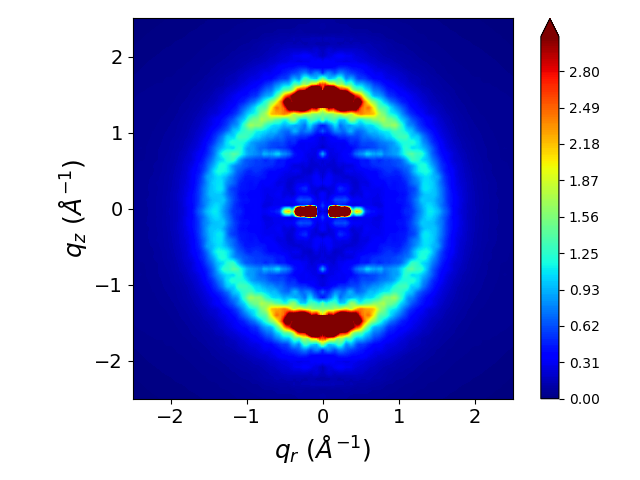
\includegraphics[width=.32\linewidth]{solvated_offset_rzplot_1.png}}%
  	\centering\begin{tabular}{@{}c@{ }c@{ }c@{ }c@{}}
  	&\textbf{1 wt\%} & \textbf{\hspace{2em}2.5 wt\%} & \textbf{5 wt\%} \\
  	\rowname{Parallel Displaced}&
  	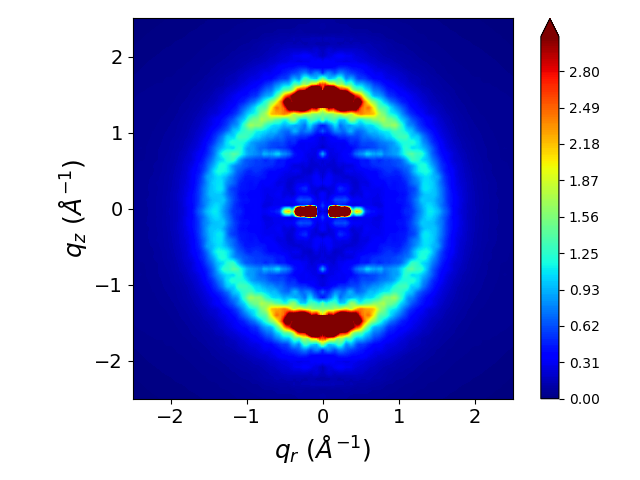
\includegraphics[width=.28\linewidth,trim={1cm 0 1.3cm 0},clip]{solvated_offset_rzplot_1.png}&
  	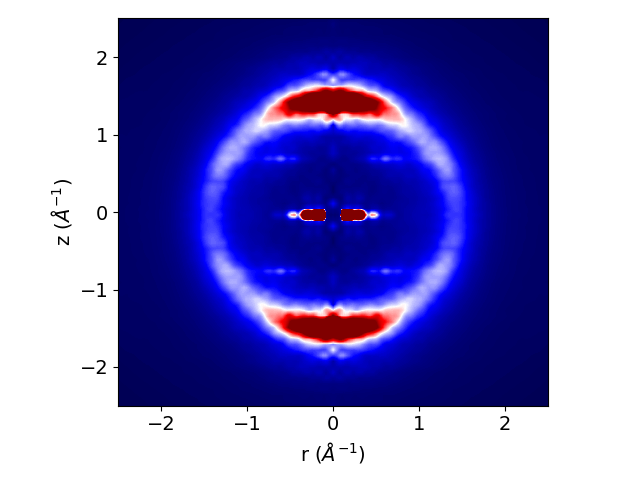
\includegraphics[width=.28\linewidth,trim={1cm 0 1.3cm 0},clip]{solvated_offset_rzplot_25.png}&
  	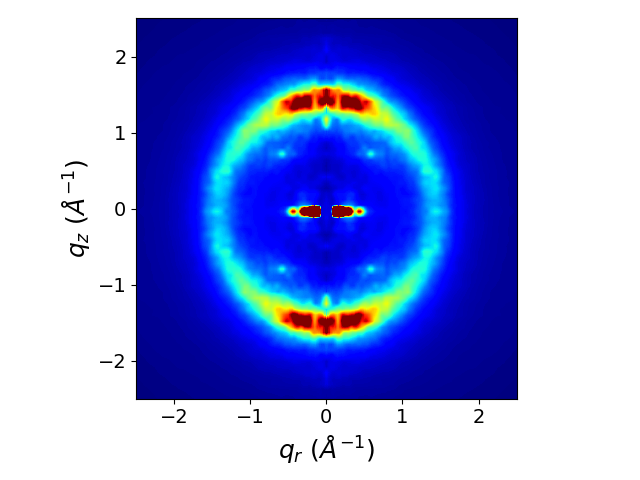
\includegraphics[width=.325\linewidth]{solvated_offset_rzplot_5.png}\\[-1ex]
  	%&\mycaption{0.2} & \mycaption{0.2} & \mycaption{0.3}\\
  	\rowname{Sandwiched}&
  	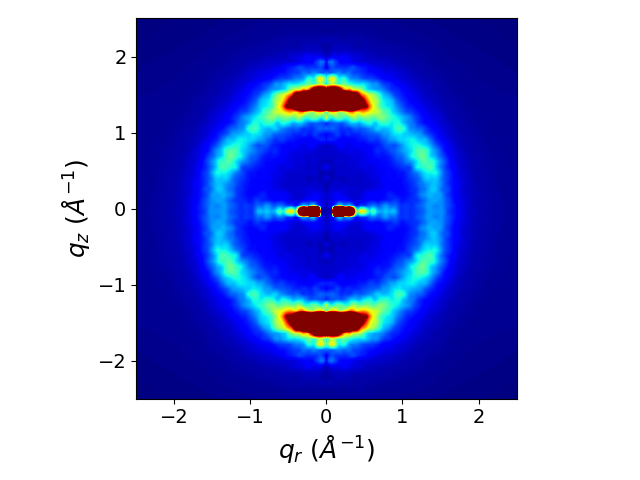
\includegraphics[width=.28\linewidth,trim={1cm 0 1.3cm 0},clip]{solvated_layered_rzplot_1.png}&
  	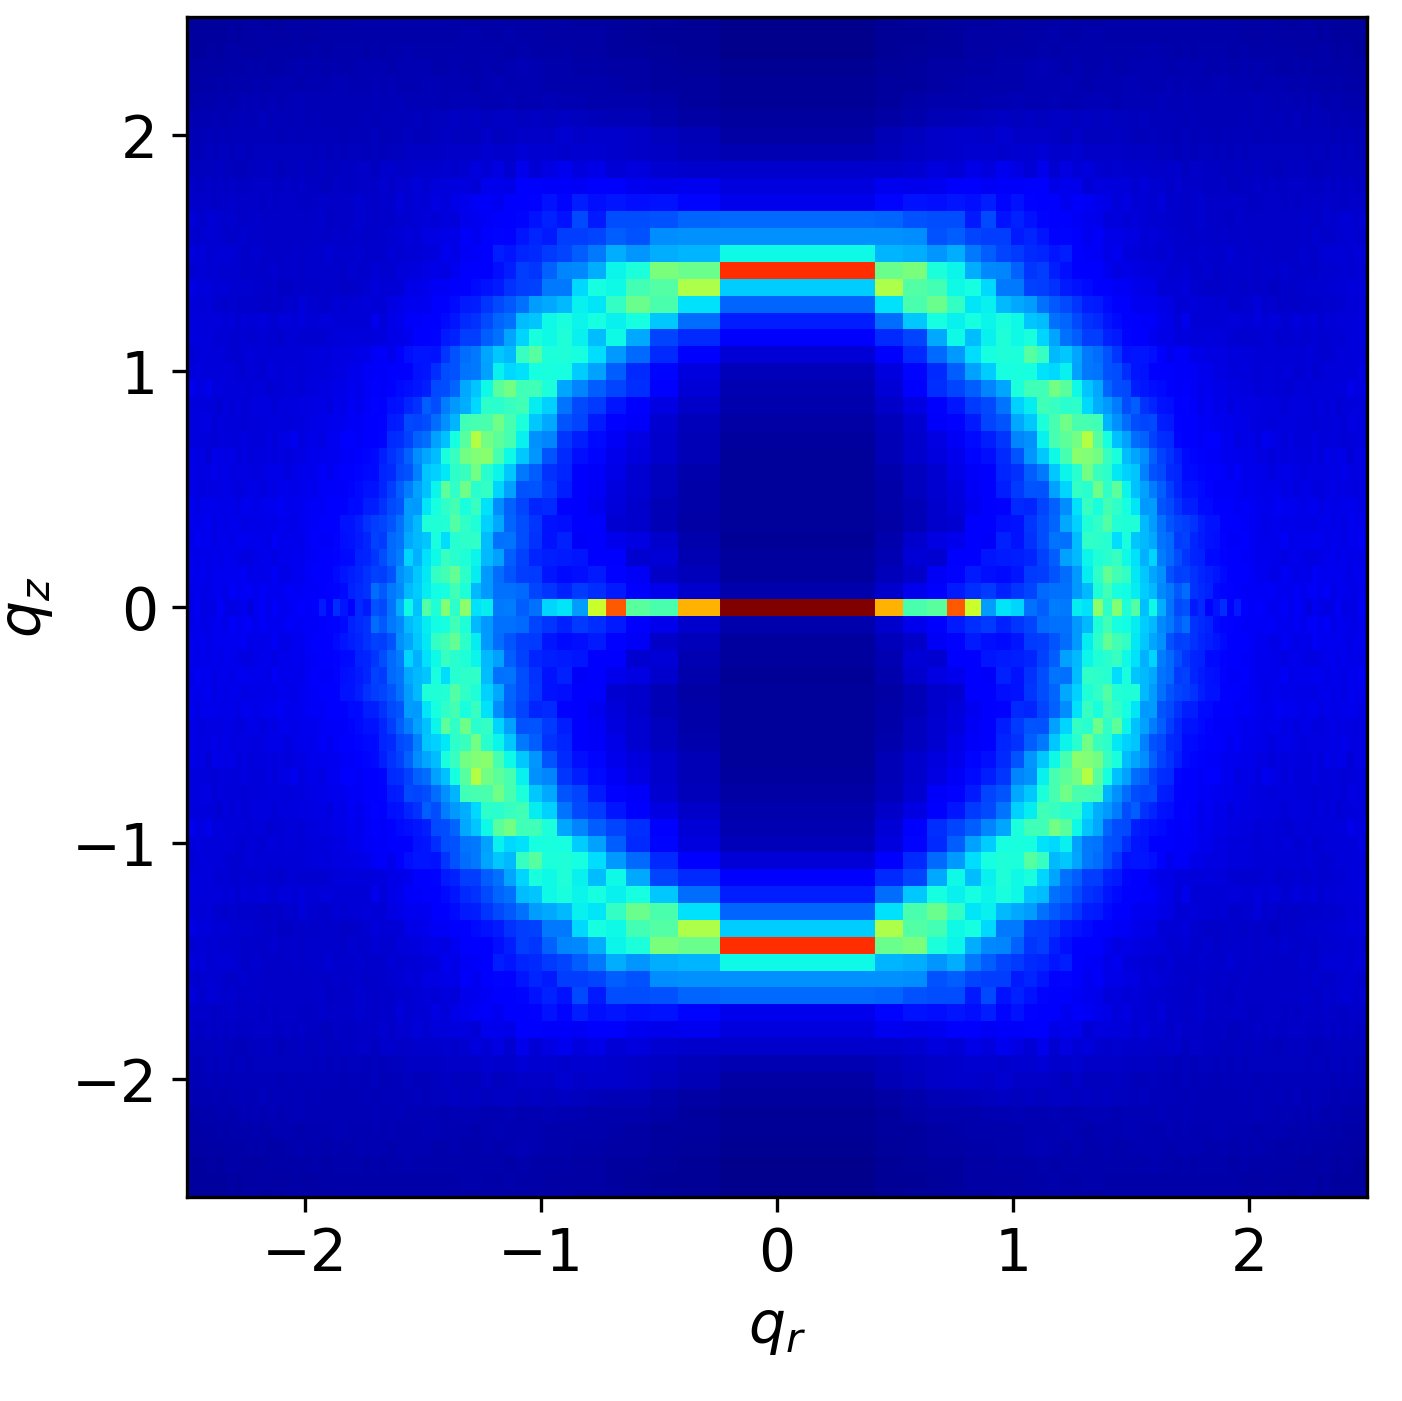
\includegraphics[width=.28\linewidth,trim={1cm 0 1.3cm 0},clip]{solvated_layered_rzplot_25.png}&
  	\includegraphics[width=.325\linewidth]{solvated_layered_rzplot_5.png}\\[-1ex]
  	%\mycaption{0.5} & \mycaption{0.6} & \mycaption{0.7} \\
  	\end{tabular}
	\caption{Simulated XRD patterns indicate that systems with added water
		are not as structured as the dry systems. As increasing amounts of water are 
		added to both systems, R-$\pi$ fades. When 2.5 wt\% water is added to the
		sandwiched system, R-$\pi$ gains back some intensity, but its magnitude is not
		greater than the dry system. R-spots also disappears as water is added. It is
		absent in all parallel displaced simulations, but fades gradually as water is
		added to the sandwiched configuration.}%
  \label{fig:solvation}

  \end{figure}
 
  In all cases, water disrupts structuring of the model.  When we add water to
  the system, the intensity of the reflections decrease. In systems built with 5
  wt\% water, R-$\pi$ and R-spots become nearly indistinguishable from R-alkanes.

  In systems built with 5 wt\% water, the pore region becomes filled with
  water. We plotted the number density of components in this system. As with the 
  dry systems, we see a gradual compositional transition from hydrophilic to hydrophobic.  
  We see that the pores become a mixture of water molecules and sodium ions (Fig.
  \ref{fig:water_density}). 
  
  The membrane swells when we introduce water. The location of maximum head
  group density shifts from 0.35 to 0.62 nm and from 0.44 to 0.61 nm in the
  parallel displaced and sandwiched configurations respectively. Again, we
  observe the existence of ions, head groups and water outside the pore region,
  however in the hydrated system, the head groups drift beyond 1.5 nm from the
  pore center. In the dry systems, head groups did not wander beyond 1.4 nm from
  the pore center. Both observations suggest that water pushes all components
  radially outward from the pore center, characteristic of a swelling process.
  The plots of $g(x,y)$ for dry and wet systems are compared in
  Figure~\ref{fig:solvated_correlation}. They further illustrate how the system
  swells in the presence of water. This system is a closer representation
  of the H\textsubscript{II} phase which is typically synthesized with ca. 8 wt\%
  water. Further investigation of hydrated systems can help unravel the
  mechanisms for selective transport in separations of aqueous solutions. 

  % BJC: unsure where or if this paragraph fits
  % BJC: Probably as the last paragraph of this section
  Water is not necessary to maintain an ordered pore structure. We do not
  eliminate the possibility that water is necessary in order to drive
  self-assembly, but studying the mechanisms of self-assembly is beyond the
  scope of this work. According to our model, once the system has formed the
  Col\textsubscript{h} phase, adding water only drives disorder of the pore
  structure. In the true equilibrium configuration, if water exists, it is
  primarily confined to the pore region where there is no driving force for
  aggregation of water molecules. In the case of trace water, water molecules
  will be too sparse to form a hydrogen bonding network.

  \begin{figure}
  \centering 
  \begin{subfigure}{0.45\textwidth}
        \includegraphics[width=1\linewidth]{offset_solvated_density.png}
        \caption{Parallel Displaced}
        \label{fig:offset_solvated_density}
  \end{subfigure}
  \begin{subfigure}{0.45\textwidth}
        \includegraphics[width=1\linewidth]{layered_solvated_density.png}
        \caption{Sandwiched}
        \label{fig:layered_solvated_density}
  \end{subfigure}
  \caption{Water fills the membrane pores in the parallel displaced (a) and
	  sandwiched (b) configurations. Head groups in the sandwiched configuration sit
	  closer to the pore center than they do in the parallel displaced configuration.
	  Both systems are composed primarily of water close to the pore center.}
  \label{fig:water_density}
  \end{figure}

  %BJC: this may be okay to push to supplemental
  \begin{figure}
  \centering
  \begin{subfigure}{0.47\textwidth}
        \includegraphics[width=1\linewidth]{layered_xy_correlation.png}
        \caption{Sandwiched, Dry}
        \label{fig:layered_xy_correlation_comparison}
  \end{subfigure}
  \begin{subfigure}{0.47\textwidth}
        \includegraphics[width=1\linewidth]{layered_solvated_xy_correlation.png}
        \caption{Sandwiched, Solvated}
        \label{fig:layered_solvated_xy_correlation}
  \end{subfigure}
  \begin{subfigure}{0.47\textwidth}
        \includegraphics[width=1\linewidth]{offset_xy_correlation.png}
        \caption{Parallel Displaced, Dry}
        \label{fig:offset_xy_correlation_comparison}
  \end{subfigure}
  \begin{subfigure}{0.47\textwidth}
        \includegraphics[width=1\linewidth]{offset_solvated_xy_correlation.png}
        \caption{Sandwiched, Solvated}
        \label{fig:offset_solvated_xy_correlation}
  \end{subfigure}
  \caption{$g(x,y)$ of monomer head groups illustrates how the pores
	  swell in the presence of water.}~\label{fig:solvated_correlation}
  \end{figure}

  \subsection{Model Ionic Conductivity Measurements}

  We used the equilibrated parallel displaced system in the ordered pore basin
  to calculate ionic conductivity since its structure is the closest match to
  experiment. The model gives reasonable estimates of ionic conductivity when
  compared to experiment.  We compare calculated values of ionic conductivity
  obtained using the Nernst-Einstein relation and Collective Diffusion model in
  Figure~\ref{fig:conductivity}. The two methods agree with each other within
  error, although the uncertainty obtained using the Collective Diffusion model
  is much higher. We require much longer simulations to lower the uncertainty,
  however it is not feasible to do so with a large system. We will only use the
  Nernst-Einstein relation in future calculations of this type. 

  The calculated values of ionic conductivity are higher than experiment by an
  order of magnitude. One can justify the reason for this result by considering
  the real system studied experimentally. The ionic conductivity measurement to
  which we are comparing was done with a \SI{80}{\micro\metre} thick film, nearly
  10,000 times thicker than our simulated system. The thick film is likely
  imperfectly aligned and has defects leading to non-contiguous pores. It has
  been shown that there is a large dependence of ionic conductivity on the
  alignment of the pores. The ionic conductivity of an isotropically aligned film
  is ca. 85 times lower than that of a nearly aligned film referenced
  here~\cite{feng_scalable_2014}. We hypothesize that a thin, perfectly aligned
  film would have a value of ionic conductivity in closer agreement with our
  model.
   
  \begin{figure}
        \centering
        \includegraphics[width=0.5\linewidth]{IC_offset.png}
        \caption{The collective diffusion model and the nernst-einstein relation yield
        agreeing values of ionic conductivity. Both methods give calculated
        values of ionic conductivity an order of magnitude higher than the experimental
        value.}
        \label{fig:conductivity}
  \end{figure}

  \subsection{Effect of Crosslinking}\label{section:xlink}

  The system's structure and physical characteristics did not change
  significantly when we applied the cross-linking algorithm to the equilibrated
  parallel-displaced configuration in the ordered pore basin. We simulated
  the cross-linked system in the NPT ensemble for 100 ns. After the system is
  cross-linked, the distance between pores shrinks by 0.4 \AA~and the distance
  between layers increases by 0.04 \AA. All major features are still present in
  the simulated XRD patterns, however at lower intensities
  (Fig.~\ref{fig:rzplot_xlink}). We calculated the ionic conductivity using the
  Nernst-Einstein relation and found that it is lower in the cross-linked system
  (Fig.~\ref{fig:IC_xlink}).
  %BJC: The current XRD pattern is from a 100 ns simulation. I am running it out
  % longer to get more statistics

  \begin{figure}
  \centering
  \begin{subfigure}{0.45\textwidth}
	\centering
	\includegraphics[width=\textwidth]{rzplot_xlink.png}
	\caption{}~\label{fig:rzplot_xlink}
  \end{subfigure}
  \begin{subfigure}{0.45\textwidth}
	\centering
	\includegraphics[width=\textwidth]{IC_xlink.png}
	\caption{}~\label{fig:IC_xlink}
  \end{subfigure}
  \begin{subfigure}{0.45\textwidth}
	\centering
	\includegraphics[width=\textwidth]{dbwl_xlink.png}
	\caption{}~\label{fig:dbwl_xlink}
  \end{subfigure}
  \begin{subfigure}{0.45\textwidth}
	\centering
	\includegraphics[width=\textwidth]{p2p_xlink.png}
	\caption{}~\label{fig:p2p_xlink}
  \end{subfigure}
  \caption{Applying our simulated crosslinking mechanism to an equilibrium
	  configuration causes slight changes to the system's physical and structural
	  properties. (a) Reflections produced by the cross-linked configuration are
	  faded relative to the uncross-linked system. (b) The ionic conductivity is
	  smaller relative to the uncross-linked system, but still much larger than the
	  experimental value. When the system is cross-linked, the distance between
	  layers increases (c) and the pore spacing decreases (d)}~\label{fig:xlink}
  \end{figure}
 
  \section{Conclusion}
  
%MRS6: I think we should remove the ``we learned'', and express it more in terms of the observed facts: rather than ``we learned statement X'', you can just say ``statement X''. Or ``observation Y in the simulations supports the conclusion Y''.  
  We have used a detailed molecular model of the Col\textsubscript{h} phase
  formed by Na-GA3C11 in order to study its nanoscopic structure. While there
  have been efforts to model formation of various liquid crystalline phases with
  molecular dynamics, to our knowledge there have been no studies which attempt
  to examine their structure with the same level of detail presented here.

  Evidence strongly supports that monomers stay partitioned into layers which
  stack to create pores and that each layer contains 5 monomers. We see periodic
  spacing of layers based on the z-direction correlation function, $g(z)$, of
  atoms in the tails and separately of atoms in the head groups. Systems not
  built with 5 monomers per layer result in assemblies whose pore-to-pore spacing
  is inconsistent with experiment. 

  We have explored the affect of two different $\pi$-$\pi$ stacking modes on
  the equilibrated membrane structure. Simulated diffraction patterns generated
  from MD trajectories suggest that the parallel-displaced configuration produces
  a structure with the closest match to experiment.

  We have observed a number of metastable configurations. We witnessed
  long-term stability of systems built with a varied number of monomers per layer
  as well as in different $\pi$-$\pi$ stacking configurations. We also examined
  how the structure changes based on the initial distance between layers and
  showed how systems differ when built with layers spaced 5~\AA~versus
  3.7~\AA~apart. The configuration that showed the greatest agreement with
  experiment was built in the parallel-displaced configuration, with 5 monomers
  per layer and an initial layer spacing of 3.7 \AA.  

  We characterized the environment centered around the membrane pores and
  learned that the pores are generally filled by monomer head groups and sodium
  ions. Membranes prepared in the sandwiched configuration have lower density 
  pores. We also observed that there is not a hard partition between hydrophlic
  and hydrophilic regions, rather there is a gradient.  This finding has raised
  questions about the nature of any size-exclusion separations.  

  We learned that we do not need water to create well-defined pore structures.
  Systems whose pores were filled with varying amounts of water showed a decrease
  in structuring relative to dry systems. 

  We justified that our system can reasonably estimate ionic conductivity.  Our
  calculations are about 1 order of magnitude higher than experiment, however
  that is to be expected since we are simulating a perfectly straight and
  defect-free membrane. 

  Finally, we verified that our conclusions do not change when the system is
  cross-linked by the algorithm we implemented. The diffraction pattern weakens
  relative to the uncross-linked system, the ionic conductivity drops by a factor
  of ca. 1.5, in closer agreement with experiment, the pore spacing decreases and
  the membrane becomes thicker. 

%MRS6'' isn't it 1-3 orders of magnitude lower? You cite some slower statistics, and there might be differences between lyotrpic and thermotropic, if the hydrophilic/hydrophobic effect is stronger than the effects in thermotropic fluids.
  We acknowledge that our simulated system exhibits glassy dynamics. The
  measured diffusion constants of monomers are three orders of magnitude lower
  than expected. It is possible that our equilibration procedure induces these
  types of metastable phases. It is also possible that the observed dynamics are
  characteristic of the real system. We took great care to overcome the potential
  limitations of our equilibration procedure and have come up with a structure
  that is in good agreement with experimental data.

  With the structural understanding gained by these simulations, we will
  evaluate transport of various solutes within the system. We will apply the
  knowledge gained from this study in order to suggest improvements to the
  existing system as well as to evaluate new unsynthesized LLC systems.

  \clearpage
  \bibliography{llc}

\end{document}

% LocalWords:  Nanostructured desalination biorefinement solute RO NF bruggen
% LocalWords:  polydisperse diffusivity solutes BJC ultrafiltration nanometer
% LocalWords:  ionizable pretreatment Graphene solvated Na GA zhou resel feng
% LocalWords:  ca wt mesophases al crosslinking THF nanoporous PDMS nanopores
% LocalWords:  TODO svg eps atomistically counterion nanoscopic counterions XRD
% LocalWords:  WAXS headgroups initio metastable timescales acessible leached
% LocalWords:  SAXS alkane alkanes Antechamber bccsym molcharge QUACPAC Openeye
% LocalWords:  Gromacs berendsen timescale Packmol xyz hydrophlic xy pd tshaped
% LocalWords:  KJ NVT kJ Parrinello Rahman gmx solvate polymerization FRP FRPs
% LocalWords:  crosslink binned DC MSD subharmonic matplotlib GAFF's xrd llc ab
% LocalWords:  polarizable reconcilable screenshot crosslinked uncrosslinked AA
% LocalWords:  nanofiltration permeability interfacial diamine polysulfone der
% LocalWords:  trimesoyl immiscible polymerizes etching Osuji's nanostructured
% LocalWords:  Donnan modelling nanotubes monodispersity maruyama Zeolites Col
% LocalWords:  lyotropic thermotropic png kinetically colorbar gromacs hess dr
% LocalWords:  gimp disassociate pore's barostat racemic colorbars Nernst LLCs
% LocalWords:  entropic rzplot transitioning spoel github pymbar Yelk Glaser
